% ===========================
% main.tex  (Overleaf, XeLaTeX)
% ===========================
\documentclass[11pt,a4paper]{article}

% ,,,,,,,,,,,,,,,,-
% Compiler: XeLaTeX (Overleaf Menu -> Compiler)
% ,,,,,,,,,,,,,,,,-
% IMPORTANT: Overleaf -> Menu -> Compiler -> XeLaTeX

% ,,,,,,,,,,,,,,,,-
% Mode switch
% ,,,,,,,,,,,,,,,,-
\newif\ifcamera
\camerafalse            % draft: one-column
% \cameratrue           % camera-ready: two-column

\ifcamera
  \PassOptionsToClass{twocolumn,twoside}{article}
\else
  \PassOptionsToClass{onecolumn,oneside}{article}
\fi

% ,,,,,,,,,,,,,,,,-
% Fonts
% ,,,,,,,,,,,,,,,,-
\usepackage{fontspec}
\defaultfontfeatures{Ligatures=TeX}

\IfFileExists{fonts/GoogleSans-Regular.ttf}{
  \setmainfont[
    Path=fonts/,
    UprightFont=GoogleSans-Regular.ttf,
    ItalicFont=GoogleSans-Italic.ttf,
    BoldFont=GoogleSans-Bold.ttf,
    BoldItalicFont=GoogleSans-BoldItalic.ttf
  ]{GoogleSans-Regular}

  \newfontfamily\GSMedium[
    Path=fonts/,
    UprightFont=GoogleSans-Medium.ttf,
    ItalicFont=GoogleSans-MediumItalic.ttf
  ]{GoogleSans-Medium}

  \newfontfamily\GSSemiBold[
    Path=fonts/,
    UprightFont=GoogleSans-SemiBold.ttf,
    ItalicFont=GoogleSans-SemiBoldItalic.ttf
  ]{GoogleSans-SemiBold}
}{
  % fallback when font files not present
  \setmainfont{TeX Gyre Heros}
  \newfontfamily\GSMedium{TeX Gyre Heros}
  \newfontfamily\GSSemiBold{TeX Gyre Heros}
}
\renewcommand{\familydefault}{\sfdefault}

% ,,,,,,,,,,,,,,,,-
% Core packages
% ,,,,,,,,,,,,,,,,-
\usepackage[
  left=25mm,
  right=25mm,
  top=34mm,
  bottom=28mm,
  includehead,
  headheight=16pt,
  headsep=11mm
]{geometry}

\usepackage{setspace}
\onehalfspacing

\usepackage{amsmath,amssymb}
\usepackage{siunitx}
\usepackage{graphicx}
\usepackage{booktabs,longtable,array,multirow}
\usepackage{float}
\usepackage{caption}
\usepackage{xcolor}
\usepackage{hyperref}
\usepackage{enumitem}
\usepackage{authblk}
\usepackage{titlesec}
\usepackage{tcolorbox}
\usepackage{fancyhdr}
\usepackage{tikz}
\usepackage{eso-pic}
\usepackage{pdflscape}
\usepackage[numbers,sort&compress]{natbib}

\hypersetup{
  colorlinks=true,
  linkcolor=black,
  citecolor=black,
  urlcolor=blue
}

\setlength{\parindent}{0pt}
\setlength{\parskip}{0.45em}
\ifcamera
  \setlength{\columnsep}{7mm}
\fi

% ,,,,,,,,,,,,,,,,-
% Section typography
% ,,,,,,,,,,,,,,,,-
\titleformat{\section}{\GSSemiBold\large}{\thesection}{0.6em}{}
\titleformat{\subsection}{\GSSemiBold\normalsize}{\thesubsection}{0.6em}{}
\titleformat{\subsubsection}{\GSMedium\normalsize}{\thesubsubsection}{0.6em}{}

% ,,,,,,,,,,,,,,,,-
% Utility macros
% ,,,,,,,,,,,,,,,,-
\newcommand{\email}[1]{\href{mailto:#1}{\texttt{#1}}}
\newcommand{\DataCheck}[1]{\textcolor{red!80!black}{\textbf{[DATA CHECK: #1]}}}
\newcommand{\Verify}[1]{\textcolor{orange!85!black}{\textbf{[VERIFY: #1]}}}
\newcommand{\Approval}[1]{\textcolor{purple!85!black}{\textbf{[APPROVAL NEEDED: #1]}}}
\newcommand{\TodoX}[1]{\textcolor{blue!70!black}{\textbf{[TODO: #1]}}}
\newcommand{\SparkPlaceholder}[1]{\textcolor{orange!85!black}{\textbf{[SPARK PLACEHOLDER: #1]}}}

\newtcolorbox{keyhighlight}{
  colback=green!5!white,
  colframe=green!45!black,
  title=Key Highlight,
  boxrule=0.7pt,
  arc=1mm
}
\newtcolorbox{reviewbox}{
  colback=yellow!8!white,
  colframe=yellow!40!black,
  title=Internal Review Flag,
  boxrule=0.7pt,
  arc=1mm
}

% Empty-check helper
\newcommand{\IfEmptyTF}[3]{%
  \if\relax\detokenize\expandafter{#1}\relax
    #2%
  \else
    #3%
  \fi
}

% ,,,,,,,,,,,,,,,,-
% Header branding band + logos (always on)
% ,,,,,,,,,,,,,,,,-
\newcommand{\HeaderBandDepth}{18mm}
\newcommand{\LogoHeight}{9.8mm}

% Define first, then set values (DON'T \renewcommand before definition)
\newcommand{\LogoLeftFile}{logos/bimotech_logo.png}
\newcommand{\LogoCenterFile}{logos/ESA_logo_2020_Deep.png}
\newcommand{\LogoRightFile}{logos/arianegroup_0.png}

\newcommand{\ApplyHeaderBranding}{
  % subtle gray gradient mask on every page (background)
  \AddToShipoutPictureBG{%
    \begin{tikzpicture}[remember picture,overlay]
      \shade[top color=black!13,bottom color=black!4]
        (current page.north west) rectangle
        ([yshift=-\HeaderBandDepth]current page.north east);
    \end{tikzpicture}
  }
  % logos (foreground)
  \AddToShipoutPictureFG{%
    \begin{tikzpicture}[remember picture,overlay]
      % Left logo
      \node[anchor=north west, xshift=8mm, yshift=-4mm]
        at (current page.north west)
        {\includegraphics[height=\LogoHeight,keepaspectratio]{\LogoLeftFile}};

      % Center logo
      \node[anchor=north, yshift=-4mm]
        at (current page.north)
        {\includegraphics[height=\LogoHeight,keepaspectratio]{\LogoCenterFile}};

      % Right logo
      \node[anchor=north east, xshift=-8mm, yshift=-4mm]
        at (current page.north east)
        {\includegraphics[height=\LogoHeight,keepaspectratio]{\LogoRightFile}};
    \end{tikzpicture}
  }
}

\AtBeginDocument{\ApplyHeaderBranding}

% ,,,,,,,,,,,,,,,,-
% Page style
% ,,,,,,,,,,,,,,,,-
\pagestyle{fancy}
\fancyhf{}
\fancyhead[L]{\footnotesize\GSMedium WAMS 2026 -- Paper \#68}
\fancyhead[R]{\footnotesize\GSMedium Lunar Metallurgy / RHEA-HEA-Ni Framework}
\fancyfoot[C]{\footnotesize\thepage}
\renewcommand{\headrulewidth}{0pt}
\renewcommand{\footrulewidth}{0pt}

% ,,,,,,,,,,,,,,,,-
% Title + author block
% ,,,,,,,,,,,,,,,,-
\title{\GSSemiBold Refractory High-Entropy Alloys and Hybrid Additive
Routes for Metallurgy in Lunar Mare, Highlands and KREEP Terranes}

\author[1]{Siddhartha Yash Kovid\thanks{\email{s.kovid@bimotech.pl}}}
\author[1]{Kevin Gr\"uning\thanks{\email{k.gruening@bimotech.pl}}}
% \author[2]{First Collaborator\thanks{\email{first.collab@iapt.fraunhofer.de}}}
% \author[3]{Second Collaborator\thanks{\email{second.collab@ariane.group}}}

\affil[1]{Bimo Tech Sp.\ Z O.\ O., Wroclaw, Poland}
% \affil[2]{Fraunhofer IAPT, Hamburg, Germany}
% \affil[3]{ArianeGroup, Additive Manufacturing Department, France}

\date{}

% =================================================================
\begin{document}

\ifcamera
\makeatletter
\twocolumn[
\begin{@twocolumnfalse}
\maketitle
\begin{abstract}\small
Sustained lunar operations will depend on turning actual lunar materials, mare basalts, feldspathic highlands and KREEP-rich crust,into usable metals and components. These reservoirs offer distinct chemistries: FeO- and TiO$_2$-rich mare basalts with abundant ilmenite (FeTiO$_3$) as a source of Fe, Ti and O; plagioclase-dominated highlands rich in Al$_2$O$_3$ and CaO; and the Procellarum KREEP Terrane (PKT) and related KREEP-bearing units enriched in K, rare-earth elements, P and heat-producing U/Th. Within ESA's FIRST! programme (SPARK -- Strong Performance Alloys for Rocket Kinetics), Bimo Tech and ArianeGroup are developing RHEAs and related systems for oxygen-rich preburners and other high-temperature propulsion components. These alloys are produced on Earth via vacuum melting, powder metallurgy and hybrid additive/subtractive routes (SLM/DED plus near-net-shape machining), and tested up to $\sim$1\,200~$^\circ$C for strength retention, oxidation resistance and microstructural stability in engine-relevant environments. This contribution shows how such Earth-qualified RHEAs and processes form a direct stepping stone toward lunar metallurgy architectures that respect real resource maps. Process windows and feedstock specifications that remain compatible when switching from terrestrial powders to ISRU-derived inputs based on mare-type basalt (Fe--Ti--rich) or highlands-type anorthosite (Al--Ca--rich). Concepts for blending ISRU metals (Al, Ti, Fe, Mg, Ca from regolith and debris) with refractory bases to produce graded components that combine high-temperature strength, oxidation resistance and, where needed, radiation shielding or KREEP-derived functional layers. A digital manufacturing toolkit (DoE + surrogate models) to predict density, defects and microstructure from process parameters, reducing empirical trials when adapting to different terranes (mare, highlands, PKT / South Pole--Aitken rim). We present current SPARK data (TRL 3--4) together with a TRL roadmap toward a modular metallurgical station for the Moon, aligned with ESA PhiLab and E3P priorities and designed to close material loops rather than ship every kilogram from Earth.
\end{abstract}
\vspace{0.4em}
\end{@twocolumnfalse}
]
\makeatother
\else
\maketitle
\begin{abstract}\small
Sustained lunar operations will depend on turning actual lunar materials, mare basalts, feldspathic highlands and KREEP-rich crust,into usable metals and components. These reservoirs offer distinct chemistries: FeO- and TiO$_2$-rich mare basalts with abundant ilmenite (FeTiO$_3$) as a source of Fe, Ti and O; plagioclase-dominated highlands rich in Al$_2$O$_3$ and CaO; and the Procellarum KREEP Terrane (PKT) and related KREEP-bearing units enriched in K, rare-earth elements, P and heat-producing U/Th. Within ESA's FIRST! programme (SPARK -- Strong Performance Alloys for Rocket Kinetics), Bimo Tech and ArianeGroup are developing RHEAs and related systems for oxygen-rich preburners and other high-temperature propulsion components. These alloys are produced on Earth via vacuum melting, powder metallurgy and hybrid additive/subtractive routes (SLM/DED plus near-net-shape machining), and tested up to $\sim$1\,200~$^\circ$C for strength retention, oxidation resistance and microstructural stability in engine-relevant environments. This contribution shows how such Earth-qualified RHEAs and processes form a direct stepping stone toward lunar metallurgy architectures that respect real resource maps. Process windows and feedstock specifications that remain compatible when switching from terrestrial powders to ISRU-derived inputs based on mare-type basalt (Fe--Ti--rich) or highlands-type anorthosite (Al--Ca--rich). Concepts for blending ISRU metals (Al, Ti, Fe, Mg, Ca from regolith and debris) with refractory bases to produce graded components that combine high-temperature strength, oxidation resistance and, where needed, radiation shielding or KREEP-derived functional layers. A digital manufacturing toolkit (DoE + surrogate models) to predict density, defects and microstructure from process parameters, reducing empirical trials when adapting to different terranes (mare, highlands, PKT / South Pole--Aitken rim). We present current SPARK data (TRL 3--4) together with a TRL roadmap toward a modular metallurgical station for the Moon, aligned with ESA PhiLab and E3P priorities and designed to close material loops rather than ship every kilogram from Earth.
\end{abstract}
\fi

\textbf{Keywords:} lunar ISRU; refractory high-entropy alloys; high-entropy alloys; Ni-superalloys; additive manufacturing; digital manufacturing; terrane-aware metallurgy; SPARK

% ============================================================
\section{Introduction}

The return to the Moon under NASA's Artemis programme and ESA's European Exploration Envelope Programme (E3P) envisions sustained human presence beyond short-duration sortie missions. A permanent lunar outpost will require structural metals, thermal-management components, and radiation shielding in quantities that make full Earth-supply economically prohibitive. In-Situ Resource Utilization (ISRU) for oxygen production from regolith has reached laboratory maturity,carbothermal reactors and molten regolith electrolysis (MRE) cells have been demonstrated at the kilogram scale~\cite{Sanders2013,Sanders2025},yet the downstream question of how to turn extracted metals into qualified engineering alloys and components remains largely unaddressed. Closing this gap requires coupling real geochemical resource maps to metallurgical process design from the outset.

The lunar crust is not a single homogeneous feedstock. Jolliff et al.~\cite{Jolliff2000} established a three-terrane geochemical framework based on Lunar Prospector Gamma Ray Spectrometer (LP-GRS) data~\cite{Prettyman2006}: (i)~feldspathic highlands, dominated by plagioclase and rich in Al$_2$O$_3$ and CaO; (ii)~mare basaltic regions, enriched in FeO and TiO$_2$ with abundant ilmenite (FeTiO$_3$); and (iii)~the Procellarum KREEP Terrane (PKT), enriched in incompatible elements (K, rare-earth elements, Th, U). Each terrane presents a distinct extraction chemistry and therefore a different starting point for alloy design~\cite{Taylor2009,Lucey2006}. Treating all regolith as equivalent,the implicit assumption in most ISRU architecture studies,introduces systematic errors in feedstock quality estimates and downstream process sizing.

Refractory high-entropy alloys (RHEAs) have emerged as a frontier material class for extreme-temperature structural applications. Body-centred cubic RHEAs based on refractory elements (Mo, Nb, Ta, W, V, Hf, Ti, Zr, Cr) retain useful strength well above the service ceiling of conventional nickel superalloys, which suffer pronounced property degradation above $\sim$700$^\circ$C~\cite{Senkov2018,George2019,Miracle2017}. Within ESA's FIRST! initiative, part of the Future Launchers Preparatory Programme (FLPP), the SPARK project (Strong Performance Alloys for Rocket Kinetics) has screened eleven candidate compositions across two alloy families --five-element refractory HEAs (SPARK-R series) and eight-element high-entropy superalloys (SPARK-H series), together with a proprietary Ni-based superalloy (SPARK-S1) --for oxygen-rich preburner environments in staged-combustion rocket engines, where operating temperatures exceed 1\,000~K and pressures reach up to 380~bar~\cite{Alvi2022}.\footnote{Exact alloy compositions are withheld under the terms of the ESA FIRST! consortium agreement. Compositions are identified by programme designators (SPARK-R1 through SPARK-R6 for five-element refractory HEAs, SPARK-H1 through SPARK-H3 for eight-element high-entropy superalloys, and SPARK-S1 for a proprietary Ni-based superalloy). Processing parameters, phase identifications, and mechanical data are reported in full to enable process-window assessment without disclosing proprietary formulations.} These alloys are synthesized via mechanical alloying (MA, 40\,h in heptane process-control agent) followed by vacuum hot pressing (HP, 1\,500$^\circ$C / 2\,h / 30\,MPa) for rapid composition screening and densification, with transfer to laser powder-bed fusion (LPBF) and directed energy deposition (DED) planned for near-net-shape manufacture of down-selected candidates. Mechanical characterisation (mini-tensile tests at room temperature and 1\,000\,K, Brinell hardness at RT and 1\,000\,K, Vickers micro-hardness HV2) and phase analysis (XRD at each processing stage; EDS elemental mapping of powders, compacts, and remelted ingots) provide the screening data. Oxidising gas-flow testing under ERBURIK conditions ($\sim$1\,000\,K) at ArianeGroup is planned for down-selected candidates. The Earth-side process chain established in SPARK,from MA/HP screening through planned LPBF/DED manufacture to hot-section testing,provides a calibrated baseline from which lunar feedstock adaptation can proceed.

Current ISRU metal-extraction research concentrates on three routes: hydrogen reduction of ilmenite for Fe and O$_2$~\cite{Anand2012}; molten regolith electrolysis yielding Fe--Si alloys and oxygen~\cite{Sanders2025}; and molten salt electrolysis (FFC-Cambridge process) producing Al--Si alloys. Additive manufacturing of lunar regolith has been explored primarily for civil-engineering applications (sintered habitats, landing pads), but metal additive manufacturing from ISRU-derived feedstock remains largely unexplored. No published framework connects terrane-resolved geochemistry to extracted-metal quality, alloy-family selection, process-window definition (HP, LPBF, DED), and qualification logic as a single integrated chain. This is the gap that the present work addresses.

We present a terrane-aware metallurgical framework that maps LP-GRS 2$^\circ$ geochemical data through compositional data analysis (CLR transform and PCA) into three metallurgical potential indices, and links these to candidate alloy families (RHEA, HEA, Ni-superalloy) and manufacturing processes via a compatibility matrix informed by SPARK Earth-side trials. The key novelty is the integration of:
\begin{itemize}[leftmargin=1.4em]
  \item terrane chemistry stratification from orbital spectroscopy,
  \item extraction-to-alloy feasibility mapping across three resource classes,
  \item process-window transfer logic anchored in SPARK experimental baselines (MA/HP screening $\rightarrow$ LPBF/DED manufacture), and
  \item a qualification roadmap that identifies the experimental campaigns needed when adapting to different lunar feedstocks.
\end{itemize}

\begin{keyhighlight}
This manuscript presents a \textbf{transfer framework anchored in SPARK experimental data}, not a completed lunar industrial implementation. SPARK screening (MA + HP, 9 compositions, XRD/EDS/mechanical testing) is complete; down-selection to two candidates is reported. Exact compositions are withheld under the consortium IP agreement; processing parameters and properties are reported in full. Microstructural characterisation of down-selected alloys is in progress.
\end{keyhighlight}

\paragraph{European programme context.}
The framework presented here is complementary to several active European lunar-manufacturing programmes. The DLR/ESA LUNA analogue facility (Cologne, opened September 2024) provides the regolith-simulant testbed at the scale required for integrated ISRU experiments. The ESA OSIP-funded \emph{Deep Sintering of Lunar Regolith Simulants} project (Activity~4000147699, TU~Berlin, implemented March 2025) demonstrates subsurface viscous sintering at 700--950$^\circ$C on both Mare and Highland simulants, directly relevant to the paper's terrane-resolved framework~\cite{ESADeepSintering2025}. The MOONRISE flight payload (LZH and TU~Berlin, DLR/BMWK funded, scheduled for an Astrobotic CLPS landing in late 2026) will demonstrate diode-laser melting of regolith on the lunar surface~\cite{MOONRISE2024}. On the metallic ISRU side, the Metalysis FFC-Cambridge process (UK SME with ESA development contract; ESA Grand Challenge Phase~1 winner) is the European Al--Si producer reduced from regolith~\cite{Lomax2020}; the Al--Si-blended alloy concept proposed below is directly compatible with that feedstock. Hot-section validation is anchored in the DLR P8 bench at Lampoldshausen, where ArianeGroup has already qualified a fully additively manufactured combustion chamber over 14 hot fires; the Stage-2 RHEA throat-inlay test of Section~\ref{sec:roadmap} is positioned within that established infrastructure.

% ============================================================
\section{Scope, Claim Boundary, and Evidence Classes}

This paper presents a \emph{framework} connecting orbital geochemistry to alloy process-window selection, not a demonstrated lunar manufacturing capability. To maintain technical credibility, every substantive claim is classified into one of four evidence tiers: \textbf{Measured} (Earth-side data from published sources or SPARK trials), \textbf{Model-derived} (computed from measured data via standard methods), \textbf{Assumed} (expert judgement requiring future validation), and \textbf{Roadmap hypothesis} (no experimental demonstration yet). Table~\ref{tab:evidence} maps the paper's key assertions to these tiers.

% ============================================================
\section{Data Sources and Analytical Workflow}

% ,,,,,,,,,,,,,,,,,,--
\subsection{Terrane-oriented geochemical dataset}

Our primary data source is the Lunar Prospector Gamma Ray Spectrometer (LP-GRS) global elemental abundance dataset at $2^\circ\times2^\circ$ equal-area spatial resolution, compiled by Prettyman et al.~\cite{Prettyman2006}. This product provides pixel-level concentrations for six major oxides and three trace elements derived from orbital gamma-ray spectroscopy.

\begin{table}[H]
\centering
\caption{LP-GRS 2-degree dataset schema. Major oxides are reported in weight percent (wt\%); trace elements in parts per million (ppm). The U abundance is tied to Th via the empirical relation $\text{U} = 0.27\,\text{Th}$ used in the LP-GRS unmixing model~\cite{Prettyman2006} and is therefore excluded from PCA to avoid introducing a linear dependency.}
\label{tab:schema}
\small
\begin{tabular}{llrl}
\toprule
\textbf{Column} & \textbf{Unit} & \textbf{Role in pipeline} & \textbf{Transform} \\
\midrule
lat, lon & deg & spatial bin identifier & --- \\
FeO      & wt\% & PCA feature + $I_\text{FeTi}$ & CLR \\
TiO$_2$  & wt\% & PCA feature + $I_\text{FeTi}$ & CLR \\
Al$_2$O$_3$ & wt\% & PCA feature + $I_\text{AlCa}$ & CLR \\
CaO      & wt\% & PCA feature + $I_\text{AlCa}$ & CLR \\
MgO      & wt\% & PCA feature & CLR \\
SiO$_2$  & wt\% & PCA feature + penalty & CLR \\
K        & ppm  & PCA feature + $I_\text{KREEP}$ & $z$-score \\
Th       & ppm  & PCA feature + $I_\text{KREEP}$ + classifier & $z$-score \\
U        & ppm  & $I_\text{KREEP}$ only & $z$-score (not in PCA) \\
terrane  & --   & Jolliff classification & --- \\
\bottomrule
\end{tabular}
\end{table}

The global dataset comprises \textbf{11\,306 spatial pixels} covering the near-complete lunar surface. For metallurgical planning we define three operational resource classes broadly aligned with the geochemical framework of Jolliff et al.~\cite{Jolliff2000}, who identified the Feldspathic Highlands Terrane (FHT), the Procellarum KREEP Terrane (PKT), and the South Pole--Aitken Terrane (SPAT). Our simplified scheme merges SPAT into the highlands class and separates mare basaltic units from KREEP-bearing regions using the following thresholds:
\begin{itemize}[leftmargin=1.4em]
  \item \textbf{Highlands} ($n = 8{,}472$; 74.9\%): Th $\leq$ 3.5~ppm and (FeO $\leq$ 8~wt\% or TiO$_2$ $\leq$ 0.5~wt\%).
  \item \textbf{Mare} ($n = 1{,}222$; 10.8\%): FeO $>$ 8~wt\% and TiO$_2$ $>$ 0.5~wt\%.
  \item \textbf{KREEP-bearing} ($n = 1{,}612$; 14.3\%): Th $>$ 3.5~ppm.
\end{itemize}

The dominance of highlands pixels reflects the lunar far side, which is almost entirely feldspathic crust~\cite{Taylor2009}.

% ,,,,,,,,,,,,,,,,,,--
\subsection{Compositional preprocessing and PCA}

The six major oxides obey a constant-sum constraint ($\sim$97~wt\%), so we apply the Centered Log-Ratio (CLR) transform~\cite{Aitchison1986} to address the closure problem~\cite{PawlowskyGlahn2011}:
\begin{equation}
\mathrm{clr}(c_i) = \ln\!\left(\frac{c_i}{g(\mathbf{c})}\right), \quad
g(\mathbf{c}) = \left(\prod_{j=1}^{D} c_j\right)^{\!1/D},
\end{equation}
where $D = 6$. The trace elements K and Th are $z$-scored independently and appended to the CLR features, creating a hybrid metric space (log-ratio + Euclidean); CLR is retained over ILR~\cite{Filzmoser2009} for interpretability. U is excluded from PCA because the LP-GRS unmixing model ties it to Th ($\text{U} = 0.27\,\text{Th}$)~\cite{Prettyman2006}.

\paragraph{Data cleaning.}
Unmixing artifacts are clipped to physically motivated bounds (FeO~0--28, TiO$_2$~0--15, Al$_2$O$_3$~0--38, CaO~0--22, MgO~0--25, SiO$_2$~35--55~wt\%) and replaced via terrane-wise median imputation (1\,414 values clipped). Below-detection zeros (2\,859 total, predominantly highlands TiO$_2$) are replaced with terrane-wise medians rather than epsilon-clipping, which would create ${\sim}{-21}\sigma$ outliers in CLR space. Approximately 38\% of pixels have at least one modified value.

\paragraph{PCA.}
PCA~\cite{Jolliffe2002} is applied to the $11{,}306 \times 8$ feature matrix. Loadings are stabilised via 200 sign-aligned bootstrap resamples~\cite{EfronTibshirani1993} ($\sigma \leq 0.034$, median $\sigma = 0.014$). Terrane separability is quantified by the silhouette coefficient~\cite{Rousseeuw1987} (0.300, ``weak but detectable'' per Kaufman--Rousseeuw 1990) and the Davies--Bouldin Index~\cite{DaviesBouldin1979} (1.247). These metrics confirm that the three operational resource classes are statistically distinguishable in PCA space, though they overlap along continuous geochemical gradients as expected at 2$^\circ$ resolution.

% ,,,,,,,,,,,,,,,,,,--
\subsection{Terrane Metallurgical Potential Indices}

To translate geochemical composition into metallurgical relevance, we define three terrane-specific indices. All oxide and trace-element concentrations are first min-max normalized to $[0, 1]$ over the full dataset before weighting.

\textbf{Fe--Ti index} (mare basalt feedstock potential):
\begin{equation}
I_{\mathrm{FeTi}} = 0.50\,\hat{c}_{\mathrm{FeO}} + 0.40\,\hat{c}_{\mathrm{TiO_2}} - 0.10\,P_{\mathrm{imp}},
\label{eq:IFeTi}
\end{equation}
where $P_{\mathrm{imp}} = 0.6\,\hat{c}_K + 0.4\,\hat{c}_{\mathrm{Th}}$ penalizes KREEP contamination in otherwise Fe--Ti-dominated pixels. High $I_{\mathrm{FeTi}}$ identifies regions suitable for ilmenite-based iron/titanium extraction.

\textbf{Al--Ca index} (highlands structural metal potential):
\begin{equation}
I_{\mathrm{AlCa}} = 0.55\,\hat{c}_{\mathrm{Al_2O_3}} + 0.35\,\hat{c}_{\mathrm{CaO}} - 0.10\,P_{\mathrm{het}},
\label{eq:IAlCa}
\end{equation}
where $P_{\mathrm{het}}$ is the min-max-normalized absolute deviation of SiO$_2$ from its terrane mean, serving as a proxy for compositional mixing. High $I_{\mathrm{AlCa}}$ identifies feldspathic regions suitable for aluminum and calcium extraction.

\textbf{KREEP index} (incompatible-element functional potential):
\begin{equation}
I_{\mathrm{KREEP}} = 0.40\,\hat{c}_K + 0.40\,\hat{c}_{\mathrm{Th}} + 0.10\,\hat{c}_U - 0.10\,P_{\mathrm{unc}},
\label{eq:IKREEP}
\end{equation}
where $P_{\mathrm{unc}} = |\mathrm{lat}|$ (min-max normalized) is a proxy for LP-GRS counting-statistics quality (polar orbits have fewer accumulated counts). Note that U is included in $I_{\mathrm{KREEP}}$ (where its physical role as a heat-producing element is relevant) even though it is excluded from PCA (where its linear dependence on Th would be a statistical artifact). High $I_{\mathrm{KREEP}}$ flags regions with enriched incompatible elements relevant for functional layers and radiation shielding.

In the above, $\hat{c}_x$ denotes the min-max-normalized concentration of species $x$, scaled to $[0,1]$ over the full dataset. All indices are clipped to $[0, 1]$ after computation. Note that the positive weights in each index sum to 0.90 while the penalty weight is 0.10, so the theoretical maximum (all positive-weight species at maximum, zero penalty) is 0.90; the upper clip at 1.0 is never binding.

% ,,,,,,,,,,,,,,,,,,--
\subsection{Alloy-family portfolio mapping}

The alloy-family portfolio mapping takes terrane chemistry ($x_t$), feedstock quality ($q_f$), and component duty ($d_c$) as inputs, and returns a candidate alloy family ($a_f$), blend window ($b_w$), process route ($p_r$), and confidence level ($c_\ell$):
\[
\mathcal{F}(x_t,\,q_f,\,d_c)\;\rightarrow\;(a_f,\,b_w,\,p_r,\,c_\ell).
\]
This is a schematic mapping, not a closed-form equation; the decision logic is implemented as the compatibility matrix in Table~\ref{tab:compat}.

% ,,,,,,,,,,,,,,,,,,--
\subsection{Cross-functional robustness of the MACE phase-stability verdict}
\label{subsec:multihead}

The ab-initio phase-stability check used throughout this work relies on the \texttt{mace-mh-1} multi-head foundation interatomic potential~\cite{Batatia2025MACEMH1}. A reviewer is entitled to ask whether the predicted formation enthalpies, and the resulting BCC-vs-FCC-vs-Laves verdicts, depend on the particular electronic-structure reference baked into the head used for evaluation. To answer this we re-evaluated every relaxed structure under three of the seven available heads, chosen to span the range of training corpora and exchange-correlation flavours relevant to bulk inorganic crystals:

\begin{itemize}[leftmargin=1.4em]
  \item \texttt{omat\_pbe} — PBE+U on the OMAT-24 inorganic corpus. This is the default head recommended for refractory and transition-metal crystals; it is the head used to generate all formation enthalpies elsewhere in the paper.
  \item \texttt{matpes\_r2scan} — r$^2$SCAN meta-GGA on the MATPES corpus. r$^2$SCAN is materially more accurate than PBE for $3d$ magnetism, which is the principal weakness of plain PBE for Fe-bearing phases.
  \item \texttt{oc20\_usemppbe} — PBE on the OC20 catalysis corpus. This head is trained on a different chemical distribution than \texttt{omat\_pbe} and provides an independent test of whether the verdict is sensitive to the training corpus rather than the functional.
\end{itemize}

The remaining four heads target molecular chemistry ($\omega$B97M, B3LYP, SPICE) or surfaces (RGD1) and are inappropriate for bulk inorganic crystals; they are not surveyed.

For each structure we hold the \texttt{omat\_pbe}-relaxed geometry fixed and recompute the total energy and pure-element references under each head. Formation enthalpies $\Delta H_f$ are reconstructed per head from the head-specific pure-element references, so the cross-head spread reflects only the disagreement that survives this normalisation,not arbitrary offsets in the absolute energy zero. Twelve structures were evaluated: the seven random-substitution supercells of the MoNbTaTiV $\rightarrow$ Fe$_{0.5}$Ti$_{0.5}$ dilution path, three published-baseline RHEAs (MoNbTaW, MoNbTaVW, AlMo$_{0.5}$NbTa$_{0.5}$TiZr), and the two C14 Laves competitors (Fe$_2$Nb, Fe$_2$Ta). Per-structure $\Delta H_f$ values for each of the three heads and the cross-head spread (max$-$min) are tabulated in Table~\ref{tab:multihead} at the end of the paper.

\paragraph{Robustness verdict.} The three all-refractory baselines (MoNbTaW, MoNbTaVW, AlMo$_{0.5}$NbTa$_{0.5}$TiZr) agree across heads to within \textbf{0.9--1.4\,kJ/mol per atom},three orders of magnitude below the $\sim$25\,kJ/mol/atom systematic accuracy commonly cited for PBE on transition-metal compounds. For these compositions the BCC-stable verdict is robust against the choice of head. The cross-head spread grows monotonically along the dilution path as the Fe fraction increases, from 0.9\,kJ/mol/atom at $x = 0$ (no Fe) to 28\,kJ/mol/atom at $x = 100\,\text{wt\%}$ (Fe-50Ti endpoint). r$^2$SCAN consistently reports the least exothermic $\Delta H_f$ on the Fe-rich compositions, which is the expected sign of the PBE magnetic over-binding in $3d$ ferromagnets that r$^2$SCAN partly corrects. The qualitative ranking,that the dilution path is monotonically exothermic toward the Fe-50Ti endpoint, and that the C14 Laves phases (Fe$_2$Nb, Fe$_2$Ta) are deeper in $\Delta H_f$ than any BCC composition on the path,is preserved across all three heads even where the absolute magnitude diverges. The two Laves end-members carry $\Delta H_f$ spreads of 37--40\,kJ/mol/atom across heads, but the sign is consistent: all three heads agree that the Laves intermetallics are thermodynamically favoured over the BCC solid solution at the Fe-rich extreme of the path. This is the physical fact the dilution-path argument relies on, and it survives the cross-validation.

\paragraph{Implication for the paper's claims.} The cross-head analysis supports two specific statements made elsewhere. First, the BCC-vs-FCC-vs-HCP energy gaps for the three reference compositions (HfNbTaTiZr, MoNbTaTiV, ISRU blend; Section~\ref{subsec:blending}) are robust phase predictions, because the underlying $\Delta H_f$ values for the all-refractory baselines (which set the energy scale) are head-invariant. Second, the central claim of the dilution path,that the Fe-rich blend Fe$_{0.3}$Ti$_{0.3}$Al$_{0.2}$Nb$_{0.1}$Ta$_{0.1}$ is exothermic to form, not merely metastable,is supported by all three heads, even though the absolute magnitude of the exothermic depth is functional-dependent (\texttt{omat\_pbe}: $-117$\,meV/atom; \texttt{oc20\_usemppbe}: more exothermic; \texttt{matpes\_r2scan}: less exothermic but still negative on the BCC supercell). The spread is honestly reported as part of the uncertainty budget for any quantitative use of MACE-derived $\Delta H_f$ on Fe-bearing compositions. Numerical values and the data files used to construct Table~\ref{tab:multihead} are deposited at \texttt{huggingface.co/datasets/Darth-Hidious/wams2026-mace-multihead}.

% ============================================================
\section{Results}

% ,,,,,,,,,,,,,,,,,,--
\subsection{PCA terrane separation}

The PC1--PC2 projection (Figure~\ref{fig:biplot}) shows the highlands cluster as compact and well-separated, with mare and KREEP overlapping along PC1. The first three principal components capture \textbf{83.6\%} of total variance (Table~\ref{tab:variance}). Loadings and their bootstrap standard deviations are listed in Table~\ref{tab:loadings}.

\begin{table}[H]
\centering
\caption{Explained variance for the first three principal components.}
\label{tab:variance}
\begin{tabular}{lSS}
\toprule
& {Explained variance (\%)} & {Cumulative (\%)} \\
\midrule
PC1 & 53.1 & 53.1 \\
PC2 & 17.4 & 70.4 \\
PC3 & 13.2 & 83.6 \\
\bottomrule
\end{tabular}
\end{table}

\paragraph{Geochemical interpretation of principal components.}

\textbf{PC1} (53.1\% variance) captures the fundamental \textbf{highlands vs.\ mare/KREEP dichotomy},the dominant gradient in lunar crustal geochemistry. The negative loadings on Al$_2$O$_3$ ($-0.39$), SiO$_2$ ($-0.40$), and CaO ($-0.35$) place the feldspathic highlands at the negative end of this axis, reflecting the anorthositic (plagioclase-rich) composition of the ancient lunar crust. The positive loadings on FeO ($+0.31$), TiO$_2$ ($+0.37$), K ($+0.40$), and Th ($+0.42$) place mare basalts and KREEP-bearing units at the positive end, reflecting their enrichment in iron-group and incompatible elements relative to the highlands. This component rediscovers the well-established geochemical bimodality of the lunar crust~\cite{Jolliff2000,Taylor2009}.

\textbf{PC2} (17.4\% variance) is dominated by \textbf{MgO} ($+0.74$), with secondary negative loadings on CaO ($-0.39$), FeO ($-0.35$), and SiO$_2$ ($-0.31$). This axis separates mafic (Mg-rich pyroxene/olivine-bearing) lithologies from more calcic or ferroan compositions. Geologically, this distinguishes Mg-suite intrusive rocks and magnesian mare basalts from ferroan anorthosites and high-Ti mare basalts.

\textbf{PC3} (13.2\% variance) is dominated by \textbf{TiO$_2$} ($+0.61$) with opposing MgO ($-0.44$) and FeO ($-0.39$). This axis captures the well-known \textbf{high-Ti vs.\ low-Ti mare basalt} distinction~\cite{Lucey2006}: high-Ti basalts (e.g.\ Apollo~11 and~17 sites) are enriched in ilmenite, whereas low-Ti basalts (e.g.\ Apollo~12 and~15 sites) have higher MgO. This distinction is directly relevant to metallurgy because high-Ti mare pixels are the primary targets for ilmenite-based oxygen and iron extraction.

The loading vectors are shown in Figure~\ref{fig:loadings}.

\paragraph{Nonlinear validation via UMAP.}
To confirm that the terrane separation observed in PCA is not an artifact of the linear projection, we computed a UMAP embedding (Uniform Manifold Approximation and Projection; $n_{\text{neighbors}} = 30$, $d_{\min} = 0.3$) of the same 8-dimensional standardised feature space. Figure~\ref{fig:umap} shows the resulting two-dimensional manifold coloured by terrane class (left) and by $I_{\text{FeTi}}$ (right). The terranes form a continuous manifold rather than discrete clusters, with highlands occupying the dominant mass, mare as a distinct arm, and KREEP bridging the two. The $I_{\text{FeTi}}$ gradient maps smoothly onto this structure, confirming that the index captures genuine geochemical variation rather than threshold artifacts. Separability metrics in UMAP space (silhouette = 0.291, DBI = 1.089) are consistent with those from PCA (0.300, 1.247), confirming that the moderate separation reflects real geochemical gradients rather than a projection artifact of either method.

% ,,,,,,,,,,,,,,,,,,--
\subsection{Manufacturability-access mapping}

The three metallurgical potential indices are projected back onto selenographic coordinates to produce global resource maps (Figures~\ref{fig:feti}--\ref{fig:kreep}). Terrane-level summary statistics are given in Table~\ref{tab:terrane_indices}.

\begin{table}[H]
\centering
\caption{Metallurgical potential indices by terrane (mean $\pm$ 1\,s.d.). The indices are dimensionless, clipped to $[0, 1]$ with a theoretical maximum of 0.90 (positive weights sum to 0.90 in all three indices).}
\label{tab:terrane_indices}
\begin{tabular}{l
  S[table-format=1.3]@{${}\pm{}$}S[table-format=1.3]
  S[table-format=1.3]@{${}\pm{}$}S[table-format=1.3]
  S[table-format=1.3]@{${}\pm{}$}S[table-format=1.3]}
\toprule
& \multicolumn{2}{c}{$I_\text{FeTi}$}
& \multicolumn{2}{c}{$I_\text{AlCa}$}
& \multicolumn{2}{c}{$I_\text{KREEP}$} \\
\midrule
Highlands     & 0.104 & 0.034 & 0.626 & 0.076 & 0.014 & 0.026 \\
Mare          & 0.490 & 0.109 & 0.186 & 0.078 & 0.096 & 0.044 \\
KREEP-bearing & 0.307 & 0.104 & 0.225 & 0.088 & 0.385 & 0.106 \\
\bottomrule
\end{tabular}
\end{table}

The indices confirm the expected terrane--resource associations:
\begin{itemize}[leftmargin=1.4em]
  \item \textbf{Highlands} pixels score highest on $I_\text{AlCa}$ ($0.626 \pm 0.076$) and lowest on both $I_\text{FeTi}$ and $I_\text{KREEP}$, consistent with their anorthositic composition.
  \item \textbf{Mare} pixels lead on $I_\text{FeTi}$ ($0.490 \pm 0.109$), reflecting their iron- and titanium-rich basaltic fill.
  \item \textbf{KREEP-bearing} pixels have the highest $I_\text{KREEP}$ ($0.385 \pm 0.106$) and moderate $I_\text{FeTi}$ ($0.307 \pm 0.104$), because the Procellarum KREEP Terrane is geographically co-located with several major mare basins.
\end{itemize}

% ,,,,,,,,,,,,,,,,,,--
\subsection{Sensitivity of metallurgical index weights}
\label{subsec:sensitivity}

The metallurgical potential indices (Eqs.~\ref{eq:IFeTi}--\ref{eq:IKREEP}) incorporate expert-assigned weights that have not been formally optimised. To assess the robustness of terrane rankings to weight uncertainty, we performed a Monte Carlo sensitivity analysis with $n = 10{,}000$ parameter perturbations.

\paragraph{Perturbation protocol.}
For each iteration, every nominal weight $w_i$ was perturbed by drawing from a truncated normal distribution:
\begin{equation}
    w_i' = w_i \cdot (1 + \epsilon_i), \quad \epsilon_i \sim \mathcal{N}(0, \sigma^2), \quad |\epsilon_i| \leq 0.5,
    \label{eq:perturbation}
\end{equation}
where $\sigma = 0.2$ (i.e., $\pm 20\%$ standard deviation, truncated at $\pm 50\%$). After perturbation, the positive weights within each index were renormalised to preserve their nominal sum while the penalty-term magnitudes were allowed to float. For each realisation, the three indices were recomputed for all 11\,306 pixels and terrane-mean values recorded.

\paragraph{Index distributions.}
Figure~\ref{fig:monte_carlo_indices} shows the distribution of terrane-mean index values across the 10\,000 Monte Carlo realisations. Table~\ref{tab:mc_summary} reports the 5th, 50th, and 95th percentiles.

\begin{table}[H]
\centering
\caption{Monte Carlo sensitivity results: terrane-mean index values (5th / 50th / 95th percentiles) across 10\,000 weight perturbations ($\sigma = 0.20$, truncated at $\pm 50\%$).}
\label{tab:mc_summary}
\begin{tabular}{lccc}
\toprule
\textbf{Index} & \textbf{Highlands} & \textbf{Mare} & \textbf{KREEP-bearing} \\
\midrule
$I_{\text{FeTi}}$  & 0.084\,/\,0.104\,/\,0.124 & 0.448\,/\,0.490\,/\,0.531 & 0.273\,/\,0.307\,/\,0.341 \\
$I_{\text{AlCa}}$  & 0.618\,/\,0.626\,/\,0.634 & 0.172\,/\,0.186\,/\,0.201 & 0.214\,/\,0.225\,/\,0.236 \\
$I_{\text{KREEP}}$ & 0.011\,/\,0.014\,/\,0.020 & 0.087\,/\,0.096\,/\,0.105 & 0.370\,/\,0.385\,/\,0.400 \\
\bottomrule
\end{tabular}
\end{table}

\paragraph{Ranking stability.}
Across all 10\,000 realisations, the terrane rankings are perfectly stable: mare pixels maintain the highest mean $I_{\text{FeTi}}$ in 100\% of cases, highlands pixels lead on $I_{\text{AlCa}}$ in 100\% of cases, and KREEP-bearing pixels dominate $I_{\text{KREEP}}$ in 100\% of cases. No ranking flip occurred under any sampled weight perturbation.

The 90\% confidence intervals (5th--95th percentile range) are narrow relative to the inter-terrane gaps. For example, the $I_{\text{FeTi}}$ 95th percentile for KREEP (0.341) falls well below the 5th percentile for Mare (0.448), confirming that the separation is robust even under worst-case weight perturbation. Among the three indices, $I_{\text{AlCa}}$ shows the tightest distributions ($\pm 1\%$ of the median), while $I_{\text{FeTi}}$ and $I_{\text{KREEP}}$ show moderate spread ($\pm 8$--15\% of the median).

\paragraph{Per-weight sensitivity.}
Figure~\ref{fig:weight_sensitivity} maps the effect of individual weight perturbations on inter-terrane separation for each index. The dominant weights ($w_{\mathrm{FeO}}$, $w_{\mathrm{Al_2O_3}}$, $w_{\mathrm{K}}$) drive up to $\pm 25\%$ change in terrane separation at $1.5\times$ perturbation, while penalty terms ($P_{\mathrm{imp}}$, $P_{\mathrm{het}}$, $P_{\mathrm{unc}}$) have near-zero effect. This confirms that the rankings are driven by genuine geochemical contrasts rather than by the penalty calibration.

% ,,,,,,,,,,,,,,,,,,--
\subsection{Terrane-to-alloy/process compatibility}

Table~\ref{tab:compat} maps each terrane chemistry to candidate alloy families and manufacturing processes, with associated risks and evidence classes.

% ,,,,,,,,,,,,,,,,,,--
\subsection{Published process baselines for candidate alloy families}

The published literature provides calibration baselines for the processing conditions and elevated-temperature performance of RHEA systems produced by SPS. Table~\ref{tab:sps_baselines} compiles SPS and HP process windows from the literature and from the SPARK campaign for representative RHEA compositions, and Table~\ref{tab:ys_comparison} compares their tensile strength at elevated temperatures against the Ni-superalloy benchmarks.

Key observations: SPS temperatures for refractory-heavy compositions (Mo, Nb, Ta, W dominant) cluster in the 1\,500--1\,800$^\circ$C range at 50--80~MPa, with hold times of 2--20~min. Alloys containing lower-melting constituents (Hf, Ti, Zr) can be sintered at lower temperatures ($\sim$1\,300$^\circ$C). MA + SPS consistently produces finer grain sizes and higher yield strength than arc-melting for the same composition~\cite{Cao2019}. Illustrative phase-fraction calculations for two reference compositions (equimolar HfNbTaTiZr and MoNbTaTiV), computed via COST507 extrapolation, suggest single-phase BCC stability across the solid-state range (Figure~\ref{fig:rhea_stability}a,b); however, COST507 lacks binary interaction parameters for most refractory pairs, so these predictions should be treated as indicative rather than confirmatory; experimental XRD from SPARK trials and published literature~\cite{Senkov2011,Cao2019} provides the primary evidence for BCC phase stability.

\paragraph{Ab-initio cross-check.}
To complement the COST507 treatment, which lacks binary interaction parameters for most refractory pairs, we recompute the $T = 0$\,K phase competition for all three reference compositions of Figure~\ref{fig:rhea_stability} using the \texttt{mace-mh-1} foundation interatomic potential~\cite{Batatia2025MACEMH1,Batatia2022MACE}, OMAT/PBE head, on 100-atom random-substitution supercells in BCC, FCC, and HCP. Formation enthalpies relative to the pure-element ground states (Fe BCC, Al FCC, Ti/Zr/Hf HCP, Mo/Nb/Ta/V BCC) are $\Delta H_f^{\text{BCC}}(\text{HfNbTaTiZr}) = +94$~meV/atom, $\Delta H_f^{\text{BCC}}(\text{MoNbTaTiV}) = -1$~meV/atom, and $\Delta H_f^{\text{BCC}}(\text{Fe}_{0.3}\text{Ti}_{0.3}\text{Al}_{0.2}\text{Nb}_{0.1}\text{Ta}_{0.1}) = -117$~meV/atom; in all three cases BCC is preferred over FCC and HCP by 21--48~meV/atom. This is an independent ab-initio confirmation of the BCC stability claim established by SPARK XRD evidence and the published Senkov / Cao literature~\cite{Senkov2011,Cao2019}, and the result for the ISRU blend ($-117$~meV/atom) is the first quantitative indication that the proposed blend is strongly exothermic to form, not merely metastable.

The ISRU column quantifies the blending opportunity using a conservative element set: only Fe, Ti, Al, Si, and Mg are counted as lunar-extractable, since these have demonstrated ISRU extraction routes (H$_2$ reduction, MRE, FFC-Cambridge). Elements present in trace lunar minerals but lacking demonstrated extraction processes (e.g.\ Zr, Cr) are counted as Earth-supplied.

For equimolar HfNbTaTiZr, only Ti is lunar-sourced ($\sim$8~wt\%). For AlMo$_{0.5}$NbTa$_{0.5}$TiZr,the most promising published RHEA for the 800--1\,000$^\circ$C regime (2\,000~MPa at RT, 745~MPa at 1\,000$^\circ$C, density 7.4~g/cm$^3$~\cite{Senkov2018}),Al and Ti together provide $\sim$19~wt\% from ISRU. Alloys composed entirely of heavy refractories (MoNbTaW, MoNbTaVW) have 0\% lunar extractability and must be shipped whole. Notably, Inconel~718 has $\sim$20\% ISRU potential (its Fe and minor Ti/Al content), but the dominant Ni and Cr fractions remain Earth-dependent.

These modest single-digit to $\sim$20\% ISRU fractions for \emph{existing} alloy compositions underscore the paper's central argument: the primary value of process-window calibration (SPARK) is not to reproduce these exact compositions on the Moon, but to establish the HP/SPS parameter space within which \textbf{new blends},dominated by ISRU-derived Fe--Ti or Al--Si, supplemented with smaller Earth-shipped refractory additions,can be explored with predictive confidence rather than trial-and-error.

Published data compiled from the Senkov--Miracle mechanical property database~\cite{SenkovMiracleData2018,Senkov2018,Senkov2011}. FFC-Cambridge outputs characterised by Lomax et al.~\cite{Lomax2020}.

% ,,,,,,,,,,,,,,,,,,--
\subsection{SPARK experimental characterisation}
\label{subsec:spark_results}

Eleven compositions were modelled using Thermo-Calc CALPHAD: six five-element refractory HEA variants (SPARK-R1 through SPARK-R6, differentiated by a single additive element to a common refractory base) and three eight-element high-entropy superalloys (SPARK-H1 through SPARK-H3). A proprietary Ni-based superalloy (SPARK-S1), identified in a partner project, was included as a comparison. Nine compositions were experimentally produced via mechanical alloying (MA, 40\,h, heptane PCA) followed by vacuum hot pressing (HP, 1\,500$^\circ$C / 2\,h / 30\,MPa, except SPARK-S1 at 1\,260$^\circ$C). Arc remelting was performed on selected compositions to assess melt behaviour and segregation.

\paragraph{Phase analysis.} XRD confirmed the computationally predicted phases at each processing stage. SPARK-R1 exhibited a dominant single-phase BCC structure from MA through HP and arc remelting. The eight-element HESA compositions showed more complex phase assemblages: SPARK-H1 and SPARK-H3 exhibited BCC + MC carbide phases, while SPARK-S1 showed FCC + MC phases after HP. XRD of SPARK-H2 after heating to 1\,000$^\circ$C showed significant peak multiplication relative to the as-HP pattern, indicating phase decomposition that may contribute to embrittlement.

EDS elemental mapping (Figure~\ref{fig:spark_eds}) confirmed homogeneous distribution of all five constituents in SPARK-R1 across both HP and remelted conditions, consistent with the single-phase BCC structure. In contrast, SPARK-R3 exhibited clear segregation of one constituent to grain boundaries (Figure~\ref{fig:spark_eds}b), producing a two-phase microstructure visible in backscatter SEM. The remelted HESA ingots showed dendritic segregation with refractory-element-rich cores and lighter-element-rich interdendritic regions.

\paragraph{Mechanical properties.} Tables~\ref{tab:sps_baselines} and~\ref{tab:ys_comparison} include the SPARK results alongside published baselines. Two results are noteworthy:

(i)~SPARK-R1, a five-element BCC RHEA, exhibits an anomalous strength increase at 1\,000\,K: UTS rises from $\sim$504\,MPa at room temperature to $\sim$532\,MPa at 1\,000\,K ($+5.6\%$), accompanied by Brinell hardness of 1\,078\,HB at RT. This intermediate-temperature strengthening is characteristic of thermally activated dislocation pinning in BCC refractory HEAs~\cite{Senkov2018} and is directly relevant to the preburner operating regime (1\,000--1\,200\,K).

(ii)~All three eight-element HESA compositions (SPARK-H1, H2, H3), despite excellent hardness (500--840\,HV2) and predicted thermal stability, exhibited extreme brittleness during all processing stages. Samples fractured during demoulding; mini-tensile specimens either could not be tested or returned UTS values below 170\,MPa with negligible plastic deformation. The five-element RHEA variants SPARK-R5 and SPARK-R6 also proved brittle, with UTS of 171 and 191\,MPa respectively.

\paragraph{Down-selection.} Two candidates were selected for further development toward combustion-chamber applications: SPARK-R1, for its single-phase BCC stability, oxidation-resistant additive, and anomalous high-temperature strengthening; and SPARK-S1, a proprietary Ni-based superalloy with 1\,250\,MPa RT UTS and 510\,MPa at 1\,000\,K, combining high strength with improved ductility over the refractory HESAs.

\paragraph{Comparison with Inconel benchmark.} An Inconel specimen produced via the same HP route returned $\sim$738\,MPa (RT) and $\sim$974\,MPa (1\,000\,K) under identical mini-tensile geometry. The apparent strength increase at temperature requires cautious interpretation: it may reflect precipitation hardening ($\gamma''$ in the 600--800$^\circ$C window), specimen geometry effects, or both. At 1\,000\,K, Inconel ($\sim$974\,MPa) outperforms SPARK-R1 ($\sim$532\,MPa); however, the SPARK-R1 trend --maintaining or gaining strength at temperature --suggests a performance crossover at higher temperatures where Ni-superalloy degradation accelerates. Confirming this crossover requires tensile data at 1\,200--1\,500\,K, planned for the next campaign.

% ,,,,,,,,,,,,,,,,,,--
\subsection{Differentiable AM-process screen for the down-selected SPARK alloys}
\label{subsec:am_screen}

The HP/SPS process windows of Section~\ref{subsec:spark_results} qualify the two down-selected compositions in the consolidation lane. The subsequent qualification lane, near-net-shape additive manufacturing by laser-powder-bed fusion (LPBF) or directed energy deposition (DED), introduces a separate set of constraints on the alloy: the melt-pool dimensions and the cooling rates achievable at a given laser power and scan speed, the dimensionless balance between viscous, capillary, gravitational and conduction time-scales inside the pool, and the sensitivity of those quantities to drift in the input material properties. Closing the SPARK process-chain qualification therefore requires a manufacturability screen at the AM stage that uses the same alloy properties already established in the consolidation lane. We implement that screen as a differentiable closed-form melt-pool model in JAX, on which gradients with respect to every material and process input are obtained by automatic differentiation rather than by finite differencing. The implementation is open and runs on a CPU; the entire screen for both alloys completes in under one minute.

\paragraph{Model.}
The model couples three textbook results. The first is the Rosenthal moving point-source temperature field~\cite{Rosenthal1946} on a semi-infinite substrate, regularised at the source by a small length scale $\varepsilon_R = 5\,\mu$m (numerically of order the beam radius) to avoid the $1/R$ singularity at the laser focus:
\begin{equation}
  T(x,y,z) \;=\; T_0 \;+\; \frac{\eta\,P}{2\pi\,\kappa\,R}\,
    \exp\!\left[-\frac{v}{2\alpha}\,(x + R)\right],
  \qquad
  R \;=\; \sqrt{x^2 + y^2 + z^2 + \varepsilon_R^{2}},
  \label{eq:rosenthal}
\end{equation}
where $\eta$ is the absorptivity at $1.06\,\mu$m, $P$ is laser power, $v$ is scan speed, $\kappa$ is thermal conductivity at LPBF working temperature, $\alpha = \kappa/(\rho c_p)$ is thermal diffusivity, and $T_0$ is the build-plate preheat. The moving frame has the laser at the origin scanning in $+x$; points behind the laser have $x<0$. The melt-pool length $L$, surface width $W$, and depth $d$ are extracted as the chord intercepts of the $T = T_m$ isotherm with the centerline ($y = z = 0$) for $L$, the $y$-axis at $x = z = 0$ for $W$, and the $z$-axis at $x = y = 0$ for $d$. The second result is the Hunt 1979 / Kurz--Fisher~\cite{Hunt1979,KurzFisher1986} primary dendrite arm spacing
\begin{equation}
  \lambda_1 \;=\; A_\text{KZ}\,|\dot T|^{-1/3},
  \qquad A_\text{KZ} \approx 80\;\mu\text{m}\!\cdot\!(\text{K/s})^{1/3},
  \label{eq:hunt}
\end{equation}
with $\dot T = -v\,\partial T/\partial x$ evaluated at the trailing-edge solidification front $x = -0.95\,L$ on the centerline; the coefficient $A_\text{KZ}$ is the Kurz--Fisher constant for the refractory-HEA family. The third is a dimensionless-analysis panel: Peclet $\mathrm{Pe} = vW/(2\alpha)$, Marangoni $\mathrm{Ma} = |d\sigma/dT|\,\Delta T\,W / (\rho\nu_l\alpha)$, and Bond $\mathrm{Bo} = \rho g W^2/\sigma_s$. The Bond number is the only place the gravitational acceleration $g$ enters the model; the Rosenthal field, the cooling rate, and Pe and Ma are all conduction- or convection-driven and gravity-independent. This makes the lunar comparison a one-line test: if Bo $\ll 1$ at both Earth and lunar gravity, the melt-pool geometry and microstructure are predicted to be identical at the two gravities, and the manufacturability verdict is portable to the Moon.

\paragraph{Sensitivities by automatic differentiation.}
Depth elasticities are derived from the implicit-function theorem applied to the Rosenthal field. The depth $d$ is defined as the root of $T(0,0,d) = T_m$, so for any input parameter $p$ that appears in $T$:
\begin{equation}
  \frac{\partial d}{\partial p} \;=\;
    -\,\frac{\partial T/\partial p}{\partial T/\partial z}\,\bigg|_{z=d,\;x=y=0},
  \qquad
  E_p \;=\; \frac{p}{d}\,\frac{\partial d}{\partial p}.
  \label{eq:elasticity}
\end{equation}
JAX evaluates both partial derivatives in closed form,no finite differences, no Gauss-quadrature step,which means the depth elasticities are exact within machine precision. Equation~\ref{eq:elasticity} chain-rules through $\alpha = \kappa/(\rho c_p)$ to give engineering elasticities with respect to the seven physically independent inputs $\{\eta, P, v, \kappa, \rho, c_p, \sigma\}$; the four formulas are also reproducible symbolically in any computer-algebra system and were independently checked by a separate symbolic-derivation script that asserts agreement with the JAX implementation to better than 0.5\,\% relative error on every reported quantity.

\paragraph{Inputs.}
Both SPARK candidates are screened at the same nominal LPBF point ($P = 200$\,W, $v = 0.8$\,m/s, $\sigma = 50\,\mu$m beam, $T_0 = 300$\,K), so the comparison is alloy-driven and not process-tuned. Material properties are taken from the consolidation-lane data of Section~\ref{subsec:spark_results}: SPARK-R1 = CrMoTaWV equimolar with $\rho = 11\,450$\,kg/m$^3$ (in-house Phase-2 measurement, 0.03\,\% agreement against the rule-of-mixtures estimate), $\kappa = 39.5$\,W/(m\,K) at LPBF working temperature (room-temperature value multiplied by $1.6\times$ to capture the high-temperature lattice-distortion uplift typical of refractory HEAs, calibrated against the published values for HfNbTaTiZr and MoNbTaW), $c_p = 221$\,J/(kg\,K) from the Dulong--Petit limit divided by mean molar mass, and $T_m = 2849$\,K from rule-of-mixtures. SPARK-S1 = HESA-2 with the experimentally produced 9-element $\gamma$--$\gamma'$ Ni--Co-base atomic composition (proprietary; characterised in SPARK Phase-2 internal documentation, available to qualified reviewers on request): the elevated $\gamma'$-former (Al + Ti) fraction puts the alloy outside the Inconel-718 reference range; rule-of-mixtures Vegard atomic volumes on the proprietary at\% composition yield $\rho = 7\,605$\,kg/m$^3$ rather than the 8\,200 of Inconel-718, mass-weighted pure-element $c_p$ at 1\,000\,K gives 580\,J/(kg\,K), $\kappa$ is taken at 21\,W/(m\,K) (midpoint of the published Mar-M-247 and Inconel-718 values at LPBF working temperature for comparable Al + Ti content), and $T_m = 1\,630$\,K liquidus. Both densities are anchored against SPARK Phase-2 internal measurements; the HESA-2 XRD pattern at the HP stage (Figure~\ref{fig:spark_xrd}) confirms the FCC matrix + minor MC-carbide assignment used here.

\paragraph{Outputs.}
Figure~\ref{fig:am_temperature_field} shows the top-view $T(x,y,z=0)$ field for both alloys at the nominal process point, with the $T_m$ isotherm drawn as a solid white curve. SPARK-R1 produces a compact, near-circular melt pool (153\,$\mu$m long, 87\,$\mu$m wide); SPARK-S1 produces a markedly elongated comet shape (416\,$\mu$m long, 64\,$\mu$m wide). The difference is driven by the thermal diffusivity contrast: $\alpha_\text{R1} = 1.56 \times 10^{-5}$\,m$^2$/s versus $\alpha_\text{S1} = 4.76 \times 10^{-6}$\,m$^2$/s, a factor of 3.3 lower in S1 because of the higher mass density and specific heat. The lower diffusivity means heat does not run ahead of the moving laser, the isotherm trails behind, and the pool extends along the scan direction. Figure~\ref{fig:am_cross_section} shows the longitudinal cross-section at $y = 0$: SPARK-R1's pool reaches 43\,$\mu$m deep, SPARK-S1's reaches 32\,$\mu$m. Both are above the 30\,$\mu$m layer-thickness threshold typical for refractory and Ni-superalloy LPBF powders, so both alloys are predicted to be printable at the nominal process point.

Figure~\ref{fig:am_process_map} maps the melt-pool depth across a 90$\times$90 grid in laser-power $\times$ scan-speed space. The 30-$\mu$m printability isoline traces a hyperbolic boundary $P/v \approx \text{const}$ characteristic of conduction-mode LPBF. The nominal SPARK process point ($P = 200$\,W, $v = 0.8$\,m/s) sits well above the boundary for SPARK-R1 (comfortable printability) and just above the boundary for SPARK-S1 (printable but with little margin, motivating $P$ above 200\,W or $v$ below 0.8\,m/s if pool stability becomes an issue at build scale).

Figure~\ref{fig:am_sensitivity} shows the engineering depth elasticities $E_p$ of Eq.~\ref{eq:elasticity} for the seven primary inputs. The signs are physically transparent and identical for both alloys: $\eta$ and $P$ raise the depth (more energy in), $v$, $\rho$, and $c_p$ lower it (faster scan or larger heat capacity removes energy faster), $\kappa$ has a small positive elasticity through its competing roles in $\alpha = \kappa/(\rho c_p)$, and the beam radius $\sigma$ has zero elasticity in the regularised point-source limit by construction. The magnitudes separate the two alloys cleanly: SPARK-R1 carries $|E| \approx 0.5$ on the dominant power/speed inputs ($\partial \ln d / \partial \ln \eta \approx +0.48$, $\partial \ln d / \partial \ln v \approx -0.53$), while SPARK-S1 carries $|E| \approx 0.76$ on $v$, $\rho$, and $c_p$ and $|E| \approx 0.48$ on $\kappa$ ,a 50\,\% higher sensitivity to process drift. This translates into a tighter qualification window for S1: a 10\,\% drift in input powder $\rho$ moves the pool depth by 7.6\,\% for S1 against 5.3\,\% for R1, so S1 needs commensurately tighter incoming-powder QA.

Figure~\ref{fig:am_lunar_dimensionless} reports the dimensionless analysis as a function of gravity. Pe and Ma are gravity-independent and identical at Earth and lunar $g$; both alloys sit in the Peclet-elongated, strongly Marangoni-stirred regime (Pe between 2 and 5, Ma between 800 and 1\,400). Bo is the only gravity-coupled number: for SPARK-R1, Bo drops from $4.04 \times 10^{-4}$ on Earth to $6.70 \times 10^{-5}$ on the Moon; for SPARK-S1, Bo drops from $1.77 \times 10^{-4}$ to $2.93 \times 10^{-5}$. All four values are between four and five decades below the Bo $= 1$ threshold at which gravity competes with surface tension for control of pool morphology. The conclusion is direct: at the 50--90\,$\mu$m pool width characteristic of LPBF, surface tension dominates by such a wide margin under Earth gravity that the additional weakening at lunar gravity is irrelevant. The melt-pool geometry, cooling rate, dimensionless numbers and depth elasticities are all gravity-portable from Earth to the Moon. What remains gravity-sensitive in lunar AM is the powder layer outside the melt pool,recoater spreading, particle electrostatic charging, spatter trajectories, debris evacuation,not the pool itself.

% ,,,,,,,,,,,,,,,,,,--
\subsection{Lunar terrane-resolved AM screen with MACE-derived density}
\label{subsec:am_lunar_terranes}

The screen of Section~\ref{subsec:am_screen} demonstrates that the two Earth-imported SPARK alloys remain printable on the Moon. The harder question, and the one this paper actually exists to answer, is whether the same model predicts a printable melt-pool for ISRU-derived feedstocks. Three lunar-side compositions are entered into the model: Fe$_{0.5}$Ti$_{0.5}$ (mare basalt via H$_2$ reduction of ilmenite), Al-12Si eutectic (highlands anorthosite via FFC-Cambridge), and the cross-terrane blend Fe$_{0.3}$Ti$_{0.3}$Al$_{0.2}$Nb$_{0.1}$Ta$_{0.1}$ that anchors the dilution path of Section~\ref{subsec:blending}. For the ISRU blend the density is taken from the MACE-MH-1-relaxed BCC supercell ($\rho = M_\text{total} / V_\text{relaxed} = 7\,172$\,kg/m$^3$, 100-atom random-substitution configuration), so the same ab-initio object that supplies the formation enthalpy in Section~\ref{subsec:blending} feeds directly into the AM-process screen. The two Earth-import baselines (SPARK-R1 and SPARK-S1) are retained at lunar gravity for direct cross-comparison. Per-alloy results are reported in Table~\ref{tab:lunar_terrane_am} and visualised in Figure~\ref{fig:am_lunar_terrane}.

\paragraph{Findings.} All five compositions return Bond numbers between $2.1 \times 10^{-5}$ and $6.3 \times 10^{-5}$ at lunar gravity, all between four and five decades below the surface-tension threshold; surface tension dominates uniformly, confirming that the Rosenthal conduction model is internally consistent for every alloy class at lunar $g$. The melt-pool depth at the nominal process point clears the 30\,$\mu$m printability threshold for all five: 33\,$\mu$m (mare Fe--Ti), 55\,$\mu$m (highlands Al--Si), 38\,$\mu$m (ISRU blend), 43\,$\mu$m (SPARK-R1), 32\,$\mu$m (SPARK-S1). Cooling rates are in the 2--12\,$\times$\,10$^6$\,K/s range characteristic of LPBF, and predicted dendrite spacings are sub-micron across the board (0.35--0.63\,$\mu$m), consistent with the fine-grained microstructures reported in the published AM literature for both refractory and Ni-superalloy systems.

Two terrane-specific engineering call-outs follow from the table. The first is that the highlands Al--Si feedstock has an absorptivity of $\eta = 0.20$ at the $1.06\,\mu$m wavelength of a standard fibre laser, less than half the value for the iron- or refractory-rich alloys. The melt pool is large because the model assumes $\eta = 0.20$ is the absorptivity actually achieved; in practice, attempting to print Al--Si with a $1.06\,\mu$m laser leads to incomplete fusion and ejecta. Lunar LPBF on highlands feedstock will require a shorter-wavelength source (green at 515\,nm or blue at 450\,nm), at which $\eta$ for aluminium rises by a factor of three to four. This is a hardware decision that cannot be ducked, and it follows directly from the absorptivity column of Table~\ref{tab:lunar_terrane_am}. The second is that the ISRU blend, with $\rho = 7\,172$\,kg/m$^3$ as supplied by MACE rather than by rule-of-mixtures, gives a printable pool of 38\,$\mu$m depth and a Bond number of $3.9 \times 10^{-5}$,within $\sim$15\,\% of the SPARK-R1 values, despite a $\sim$35\,\% lower density. This is the quantitative basis for the paper's central claim: the ISRU-blend alloy, designed entirely from terrane chemistry plus a small refractory addition, is predicted to print under the same LPBF parameter window already qualified for SPARK-R1, with no anticipated derating on the Moon. Numerical values, the relaxed structure files, and the JAX script are deposited at \texttt{huggingface.co/datasets/Darth-Hidious/wams2026-am-lunar-terranes}.

% ============================================================
\section{Discussion}

The results support terrane-specific manufacturing logic rather than a one-size-fits-all approach. This section traces the logic chain from geochemical prediction through process calibration to the blending concept that connects ISRU bulk metals with SPARK-qualified refractory alloy routes.

The silhouette coefficient of 0.300 should be understood in context: the terrane boundaries are threshold-based cuts on a continuous geochemical gradient, not natural clusters. Perfect separation would be suspicious given the spatial resolution (2$^\circ$ pixels blend multiple lithologies) and the gradational nature of terrane transitions. The value falls in the 0.25--0.50 range conventionally described as ``weak structure,'' yet the separability is sufficient to assign distinct metallurgical strategies with quantified confidence.

\subsection{What the PCA tells us: feedstock prediction from orbit}

The three principal components recovered from LP-GRS data rediscover the established geochemical gradients of the lunar crust,highlands vs.\ mare enrichment, mafic differentiation, and Ti variability,without prior knowledge of sample-return petrology, demonstrating that orbital spectroscopy alone provides sufficient chemical resolution for first-order metallurgical planning. The metallurgical potential indices translate these gradients into actionable resource predictions:

\begin{itemize}[leftmargin=1.4em]
  \item \textbf{Mare pixels} ($I_\text{FeTi}$ dominant) identify regions where hydrogen reduction of ilmenite or carbothermal processing can yield Fe--Ti feedstock and process oxygen~\cite{Sanders2013,Anand2012}.
  \item \textbf{Highlands pixels} ($I_\text{AlCa}$ dominant) flag anorthositic crust suited to molten regolith electrolysis or the FFC-Cambridge process, producing Al--Si structural alloys.
  \item \textbf{KREEP-bearing pixels} present a dual opportunity: co-located $I_\text{FeTi}$ and $I_\text{KREEP}$ in the Procellarum region (Table~\ref{tab:terrane_indices}) enable combined Fe--Ti extraction with recovery of high-$Z$ elements (Th, U) for radiation-shielding applications.
\end{itemize}

Crucially, these ISRU routes produce \emph{bulk metals} (Fe, Ti, Al, Si, Mg, and oxygen), not the refractory elements (Mo, Nb, Ta, W, Hf, V, Cr) that constitute RHEA compositions. The Moon's crust is depleted in siderophile and highly refractory elements relative to Earth; no known lunar extraction process yields Mo, Nb, or Ta at useful purity. This asymmetry is central to the framework's logic.

\subsection{What SPARK provides: calibrated process knowledge}

The SPARK project screened eleven compositions across two alloy families for oxygen-rich preburner components in staged-combustion rocket engines, where the benchmark material (Inconel / Monel~K500) suffers property degradation above $\sim$700$^\circ$C. The experimental campaign comprised mechanical alloying (MA, 40\,h, heptane PCA), vacuum hot pressing (HP, 1\,500$^\circ$C / 2\,h / 30\,MPa), and arc remelting, with phase analysis (XRD, EDS) at each stage and mechanical testing (mini-tensile at RT and 1\,000\,K, Vickers and Brinell hardness) on the densified compacts.

The campaign produced two principal findings. First, SPARK-R1, a five-element BCC RHEA, demonstrates single-phase BCC stability across all processing stages, homogeneous microstructure after hot pressing, and anomalous strength retention at 1\,000\,K (532\,MPa, a 5.6\% increase over the RT value of 504\,MPa). Second, the eight-element HESA compositions --despite excellent hardness (500--840\,HV2) and computational predictions of thermal stability --are too brittle for structural service, fracturing during demoulding and returning negligible ductility under tension.

For the lunar transfer framework, SPARK's deliverable is a \textbf{calibrated process chain}: powder morphology after 40\,h MA (sub-micron, confirmed by SEM), HP densification profiles (1\,500$^\circ$C / 30\,MPa / 2\,h achieving 9.4--12.9\,g/cm$^3$ across compositions), phase stability maps validated against XRD, and process--property relationships linking input chemistry to density, phase assemblage, hardness, and tensile response. Transfer to LPBF and DED for near-net-shape manufacture of SPARK-R1 and SPARK-S1 is the next programme milestone. The HP windows established here define the sintering parameter space within which input powder chemistry can be varied --including substitution of ISRU-derived Fe--Ti or Al--Si for a fraction of the refractory elements --while maintaining predictable output quality.

\paragraph{Pugh's G/B as a single-descriptor printability surrogate.}
The recently published JOM 2025 RHEA additive-manufacturability index of Oriola \emph{et al.}~\cite{Oriola2025AMI,Oriola2025LaserGlazing} establishes Pugh's $G/B$ ratio~\cite{Pugh1954} as the strongest single empirical predictor of laser-powder-bed-fusion cracking susceptibility in refractory HEAs (Pearson $r = -0.90$ against cumulative crack length on a four-alloy validation set, with $G/B$ values clustered at 0.402--0.404). Using \texttt{mace-mh-1}-derived elastic constants for all five published baselines of Table~\ref{tab:sps_baselines} plus the BCC compositions along the dilution path, we compute Voigt--Reuss--Hill polycrystalline $G/B$ values: 0.273 (HfNbTaTiZr), 0.259 (MoNbTaTiV), 0.325 (MoNbTaVW), 0.339 (AlMo$_{0.5}$NbTa$_{0.5}$TiZr), 0.364 (MoNbTaW), with Fe$_2$Nb (0.44) and Fe$_2$Ta (0.50) as Laves end-members. All published BCC baselines and dilution-path compositions sit below the Pugh ductile/brittle threshold of 0.57, in the predicted ductile regime; MoNbTaW (the 0\%-ISRU baseline) has the highest $G/B$ of the pure-refractory family and is therefore predicted to be the most cracking-prone of that family by the JOM 2025 correlation. AlMo$_{0.5}$NbTa$_{0.5}$TiZr, the 19\%-ISRU literature headline, gives $G/B = 0.339$ --- comparable to the JOM cohort, predicted ductile-printable. Full evaluation of the JOM 2025 index requires the freezing-range and Kou-CSI components, which depend on a TCHEA-grade thermodynamic database and remain future work.

\subsection{The bridge: blending ISRU bulk metals with Earth-shipped refractories}
\label{subsec:blending}

The connection between ISRU feedstock prediction (Section~5.1) and SPARK process knowledge (Section~5.2) operates through a \textbf{blending concept}.

The SPARK experimental results provide a materials-science motivation for the blending concept beyond mass savings. The eight-element refractory HESAs (SPARK-H1 through H3) exhibit hardness values of 500--840\,HV2 --among the highest reported for bulk HEA compacts --but are catastrophically brittle, rendering them unsuitable for structural applications as monolithic components. Alloying with ISRU-derived ductile-phase metals (Fe, Ti, Al) offers a potential route to improve toughness: Fe--Ti from mare ilmenite reduction could serve as a ductile BCC matrix into which small fractions of refractory elements are dissolved or dispersed as strengthening phases, analogous to the oxide-dispersion-strengthened (ODS) steel concept but using HEA strengtheners rather than oxide particles. The SPARK brittleness data thus reframes the blending question from ``how much Earth mass can we save?'' to ``can ISRU-derived ductile phases solve the toughness problem that limits monolithic refractory HESAs?''

The blending logic proceeds in three steps:

\begin{enumerate}[leftmargin=1.4em]
  \item ISRU extraction at a given terrane produces bulk metal powder (e.g.\ Fe--Ti from mare ilmenite, Al--Si from highlands anorthosite).
  \item This ISRU-derived powder is blended with small quantities of Earth-shipped refractory elements (Mo, Nb, Ta, W) to form a feedstock compatible with the SPARK-calibrated process chain.
  \item The blended feedstock undergoes HP screening to verify sinterability and phase stability, followed by LPBF or DED manufacture of near-net-shape components using SPARK-calibrated build parameters. The process--property relationships from SPARK predict whether acceptable density and microstructure will be achieved, reducing the experimental campaign needed for each new composition.
\end{enumerate}

In early lunar operations, the refractory fraction is entirely Earth-supplied,but because refractories constitute a minor mass fraction of the final component (typically 5--30~wt\% depending on the alloy system and duty), the total Earth-import burden is sharply reduced compared to shipping finished parts. A mare-derived Fe--Ti powder blended with $\sim$10~wt\% Earth-supplied Mo and Nb, screened via HP and then manufactured by LPBF or DED through SPARK-calibrated process windows, could yield a structural alloy with high-temperature capability exceeding that of pure ISRU iron,while importing only a tenth of the component mass from Earth.

An important caveat applies to the blending concept: adding lower-melting ISRU-derived elements (Al, Si, and to a lesser extent Ti) to refractory bases (Mo, Nb, Ta, W) depresses the solidus temperature, potentially compromising the high-temperature strength that motivates RHEA selection. This trade-off suggests a \textbf{graded architecture} for lunar components: ISRU-dominated alloys (Fe--Ti, Al--Si) for structural applications below $\sim$800$^\circ$C, blended compositions (ISRU base + 10--30~wt\% Earth-shipped refractories) for intermediate-temperature service, and Earth-pure RHEAs reserved for the most demanding hot-section components (combustion chambers, nozzle throats) where temperatures exceed 1\,200$^\circ$C. The binary phase diagrams for the Fe--Ti, Al--Ti, Al--Fe and Al--Ni systems (Figure~\ref{fig:phase_diagrams}) illustrate the phase fields accessible from ISRU feedstocks and help bound the compositional space for each service tier.

As ISRU extraction technology matures and diversifies beyond the first-generation Fe/Ti/Al/Si routes, the Earth-shipped fraction can progressively shrink. The metallurgical potential indices provide the planning tool: they identify which terranes offer which bulk metals, enabling mission architects to size the refractory supplement inventory against the local resource base.

\paragraph{Solute dissolution refines the blending narrative.}
Single-substitution dilute-solute calculations with \texttt{mace-mh-1} into the relaxed BCC matrices of HfNbTaTiZr and MoNbTaTiV show that, at infinite dilution, Fe and Ti are both \emph{energetically uphill} solutes in the pure refractory matrices ($E_{\text{sub}}(\text{Fe}) = +0.19$~eV in HfNbTaTiZr; $+0.30$~eV in MoNbTaTiV; $E_{\text{sub}}(\text{Ti}) = +0.09$ and $+0.35$~eV respectively), with only Al favourable ($-0.72$~eV in HfNbTaTiZr; $-0.09$~eV in MoNbTaTiV). The simplest reading of the blending concept --- ``Fe-Ti from ISRU dissolves into a refractory matrix'' --- is therefore not supported by the dilute-solute thermodynamics. The favourable formation enthalpy of the ISRU blend Fe$_{0.3}$Ti$_{0.3}$Al$_{0.2}$Nb$_{0.1}$Ta$_{0.1}$ ($\Delta H_f = -117$~meV/atom) originates from bulk Fe-Ti-Al chemistry, in which the refractory elements act as solid-solution strengtheners of an ISRU-dominated matrix rather than as the matrix itself. This refinement is consistent with, and strengthens, the graded-architecture proposal above: pure RHEAs for hot sections, ISRU-dominated blends for medium-temperature service.

\subsection{Broader implications}

The framework presented here does not claim to solve lunar manufacturing; rather, it provides a structured methodology for deciding \emph{where on the Moon to extract what}, \emph{which bulk metals become available}, and \emph{how to combine them with Earth-supplied elements} using process windows calibrated in SPARK. This terrane-aware approach reduces the combinatorial search space for future ISRU demonstration missions and provides quantitative site-selection metrics that complement terrain trafficability and volatile-access considerations in landing-site trade studies. Once SPARK trials yield validated process--property relationships across the HP$\rightarrow$LPBF/DED chain, these relationships can inform how shifting from terrestrial to blended ISRU/refractory powder chemistry will affect density, defect populations, and microstructure,reducing the number of physical experiments needed during proxy-feedstock demonstration campaigns.

% ============================================================
\section{Economic Considerations}
\label{sec:economics}

The terrane-aware metallurgy framework has direct implications for lunar infrastructure economics. This section develops a parametric cost model that maps the decision space for ISRU-integrated manufacturing without claiming precision on inherently uncertain future costs. All economic projections are classified as \textbf{Roadmap hypothesis} (Tier~R) per Table~\ref{tab:evidence}.

\subsection{ISRU Mass Leverage Ratio}
\label{subsec:imlr}

We define the \emph{ISRU Mass Leverage Ratio} (IMLR) as the ratio of final component mass to Earth-shipped feedstock mass:
\begin{equation}
    \text{IMLR} = \frac{M_{\text{component}}}{M_{\text{Earth}}} = \frac{M_{\text{ISRU}} + M_{\text{Earth}}}{M_{\text{Earth}}},
    \label{eq:imlr}
\end{equation}
where $M_{\text{ISRU}}$ is the mass contribution from lunar-extracted metals (Fe, Ti, Al, Si, Mg) and $M_{\text{Earth}}$ is the mass of Earth-shipped feedstock (refractory elements Mo, Nb, Ta, W, Hf, V, Cr plus any required alloying additions not extractable on the Moon).

For the candidate alloy systems in Table~\ref{tab:ys_comparison}, IMLR ranges from 1.0 (pure Earth-shipped RHEAs like MoNbTaW) to approximately 1.25 (AlMo$_{0.5}$NbTa$_{0.5}$TiZr with 19\% ISRU content). The blending concept proposed in Section~\ref{subsec:blending} targets IMLR values of 5--10 for structural applications, achieved by using ISRU-derived Fe--Ti or Al--Si as the matrix phase with 10--20~wt\% Earth-shipped refractory additions.

\subsection{Parametric Cost Model}
\label{subsec:cost_model}

The total cost $C_{\text{total}}$ to produce $N$ components of mass $M_{\text{component}}$ via ISRU-integrated manufacturing comprises launch costs, capital expenditure, and operating costs:
\begin{equation}
    C_{\text{total}} = \underbrace{C_L \cdot M_{\text{Earth}} \cdot N}_{\text{Launch}}
    + \underbrace{C_{\text{cap}}}_{\text{Capital}}
    + \underbrace{C_{\text{op}} \cdot M_{\text{ISRU}} \cdot N}_{\text{Operations}},
    \label{eq:total_cost}
\end{equation}
where $C_L$ is the cost to deliver 1~kg to the lunar surface (\$/kg), $C_{\text{cap}}$ is the capital cost of the ISRU metallurgical station including launch mass (\$), $C_{\text{op}}$ is the operating cost to extract and process 1~kg of ISRU metal (\$/kg), and $N$ is the number of components produced over the station lifetime.

The break-even condition against pure Earth-supply ($C_{\text{total}}^{\text{ISRU}} = C_{\text{total}}^{\text{Earth}}$, where $C_{\text{total}}^{\text{Earth}} = C_L \cdot M_{\text{comp}} \cdot N$) yields, after substituting $M_{\text{Earth}} = M_{\text{comp}} / \text{IMLR}$:
\begin{equation}
    C_{\text{op}} < C_L - \frac{C_{\text{cap}}}{N \cdot M_{\text{ISRU}}}.
    \label{eq:breakeven}
\end{equation}
This inequality defines the \emph{viable parameter space} for ISRU-integrated manufacturing: the per-kilogram operating cost of ISRU extraction must be less than the launch cost minus the amortised capital burden. Notably, break-even depends on production volume $N$: higher throughput amortises capital costs and expands the viable operating cost range.

\subsection{Launch Cost Scenarios}
\label{subsec:launch_scenarios}

Table~\ref{tab:launch_costs} summarises lunar surface delivery costs across launch architectures, grounded in publicly available contract and pricing data. The wide range,spanning two orders of magnitude,reflects the rapid evolution of the launch market.

\begin{table}[H]
\centering
\caption{Lunar surface delivery cost scenarios (2026 baseline). CLPS costs are derived from NASA contract values divided by payload capacity~\cite{NASAOIG2024}. The Falcon Heavy LEO cost of \$1\,400/kg~\cite{Jones2023} is scaled by a $\sim$7$\times$ mass multiplier for trans-lunar injection, orbit insertion, and soft landing. Starship projections assume 100\,t cargo to lunar surface; fully reusable targets per Jones~\cite{Jones2023}.}
\label{tab:launch_costs}
\begin{tabular}{lp{3.4cm}cc}
\toprule
\textbf{Scenario} & \textbf{Architecture} & \textbf{$C_L$ (\$/kg)} & \textbf{Status} \\
\midrule
CLPS (small lander) & IM-1 Nova-C (\$118M / $\sim$100~kg) & ${\sim}$1\,200\,000 & Demonstrated (2024) \\
Heavy lander & FH + Griffin-class ($>$500~kg) & ${\sim}$200\,000 & Near-term \\
Starship HLS & 100\,t-class reusable & ${\sim}$50\,000 & Projected \\
Fully reusable & FH-class $\times$ 7$\times$ multiplier & ${\sim}$10\,000 & Aspirational \\
\bottomrule
\end{tabular}
\end{table}

\textit{Caveat:} The ``Starship'' and ``Fully reusable'' scenarios assume successful development of fully or partially reusable lunar landing systems. SpaceX's current LEO cost target for Starship is \$78--94/kg with partial reusability, with a long-term target of \$10/kg; lunar surface costs include the substantial delta-$v$ penalty ($\sim$6~km/s from LEO) and propellant depot operations that remain undemonstrated. These costs should be treated as bounding cases rather than planning baselines.

\subsection{ISRU Extraction Cost Estimates}
\label{subsec:extraction_costs}

Extraction cost estimates derive from NASA technology development studies. Table~\ref{tab:extraction_costs} compiles published values with their underlying assumptions. Jones~\cite{Jones2023} estimates lunar oxygen delivered in a qualified tank at \$18\,700/kg under the Falcon Heavy architecture; however, this assumes high-volume bulk delivery. At CLPS-era launch costs, the effective cost of oxygen in orbit far exceeds this figure.

\begin{table}[H]
\centering
\caption{ISRU metal extraction cost estimates. O$_2$ values from Sanders~\cite{Sanders2025} and Jones~\cite{Jones2023}; metal costs scaled from oxygen extraction as described in text.}
\label{tab:extraction_costs}
\begin{tabular}{lccc}
\toprule
\textbf{Product} & \textbf{$C_{\text{op}}$ (\$/kg)} & \textbf{Basis} & \textbf{Source} \\
\midrule
O$_2$ (from regolith) & 500\,000--2\,000\,000 & Amortised, 10-yr & Sanders 2025 \\
O$_2$ (optimistic) & ${\sim}$18\,700 & FH-era bulk delivery & Jones 2023 \\
Fe (H$_2$ reduction) & 100\,000--500\,000$^*$ & Scaled from O$_2$ & This work \\
Al--Si (MRE/FFC) & 200\,000--1\,000\,000$^*$ & Scaled from O$_2$ & This work \\
Fe--Ti (ilmenite) & 80\,000--400\,000$^*$ & High-Ti mare & This work \\
\bottomrule
\multicolumn{4}{l}{\footnotesize $^*$Extrapolated from oxygen extraction costs; treat as order-of-magnitude.}
\end{tabular}
\end{table}

Iron extraction from high-Ti mare ilmenite is projected to have the lowest cost due to the relatively simple hydrogen reduction chemistry and high ilmenite concentrations in mare regolith~\cite{Sanders2013, Anand2012}. The ``This work'' estimates scale O$_2$ extraction costs by the additional energy and processing complexity of metal reduction: Fe from ilmenite requires only H$_2$ reduction at $\sim$1\,000$^\circ$C (modest uplift), while Al--Si via MRE or FFC-Cambridge requires higher-temperature electrolysis ($\sim$1\,600$^\circ$C) and more complex cell design (2--5$\times$ uplift). These are deliberately wide ranges reflecting order-of-magnitude uncertainty.

\subsection{Break-Even Analysis}
\label{subsec:breakeven_analysis}

Figure~\ref{fig:breakeven} presents contour plots of the break-even operating cost (Eq.~\ref{eq:breakeven}) across the launch cost--production volume parameter space for two IMLR scenarios: conservative (IMLR~=~2, corresponding to $\sim$50\% ISRU content) and optimistic (IMLR~=~5, corresponding to $\sim$80\% ISRU content).

Key observations:
\begin{enumerate}[leftmargin=1.4em]
    \item At current demonstrated launch costs ($C_L \approx$ \$1M/kg), ISRU-integrated manufacturing breaks even at moderate production volumes ($N > 100$ components for IMLR~=~2; $N > 63$ for IMLR~=~5). At $N = 1{,}000$, the maximum viable operating cost reaches $\sim$900~k\$/kg, comparable to the upper range of oxygen extraction estimates in Table~\ref{tab:extraction_costs}.

    \item Counter-intuitively, the Starship-era scenario ($C_L \approx$ \$50k/kg) makes ISRU \emph{harder} to justify economically: the capital cost of the metallurgical station (\$500M) now dominates, requiring $N > 2{,}000$ components (IMLR~=~2) or $N > 1{,}250$ (IMLR~=~5) before the operating cost budget turns positive. Cheap launch undercuts the economic case for in-situ production unless capital costs fall proportionally.

    \item Higher IMLR values (more ISRU content) improve the capital amortisation rate (larger $M_{\text{ISRU}}$ per component) but require validated alloy compositions and process windows; precisely the gap that SPARK calibration addresses.

    \item The capital cost term dominates at low production volumes and low launch costs alike, emphasising the importance of designing modular, multi-purpose metallurgical stations rather than single-product facilities, and of reducing station mass through technology maturation.
\end{enumerate}

% ,,,,,,,,,,,,,,,,,,--
\subsection{Economic Amortisation via Dual-Purpose Mass}
\label{subsec:dual_purpose}

The break-even analysis above assumes that the Earth-shipped refractory fraction ($M_{\text{Earth}}$) is transported as dead-weight cargo: raw powder with no function other than serving as alloy feedstock. This is the worst case economically: every kilogram of refractory incurs the full launch penalty $C_L$. We now introduce a \textbf{dual-purpose mass} concept that eliminates this penalty entirely.

\paragraph{The gravity-margin dividend.}
Earth-launched spacecraft structures are sized for launch loads: quasi-static accelerations of 3--6$g$ axial plus severe acoustic and random vibration environments during ascent through maximum dynamic pressure (Max-Q)~\cite{Sarafin1995}. Once a lander reaches the lunar surface, the gravitational load drops to 0.16$g$---roughly 20--40$\times$ below the design loads. Landing struts, structural frames, thermal shields, and mounting brackets transition from load-bearing members to dead weight. The structural mass fraction of a lunar lander is typically 15--25\% of landed mass, representing tens to hundreds of kilograms of high-performance metal that serve no further purpose after touchdown.

\paragraph{Dual-purpose mass concept.}
Instead of shipping raw refractory powder as dead-weight cargo, we propose manufacturing critical spacecraft structural components (landing struts, mounting brackets, thrust-structure frames) from concentrated RHEA compositions, drawing on the broad compositional design space mapped by Gorsse et al.~\cite{Gorsse2017}. These components fulfil their primary mission duty (surviving launch loads, providing structural integrity during transit and landing) and are then \textbf{cannibalized} after landing to serve as a master-alloy seed for ISRU-blended manufacturing. The refractory elements (Mo, Nb, Ta, W) arrive on the lunar surface not as inert cargo but as functional hardware whose transport cost is entirely amortised by its primary mission role.

\paragraph{Master alloy dilution.}
The cannibalized RHEA components are not recast as pure refractory parts. Following the classical master-alloy paradigm used in grain refinement of light alloys~\cite{Easton1999}, they are diluted with locally extracted bulk metals (Fe--Ti from mare ilmenite reduction or Al--Si from FFC-Cambridge processing) per the blending concept of Section~\ref{subsec:blending}. A single 100~kg RHEA landing strut, for example, acts as a master alloy seed for 400~kg of ISRU iron, yielding 500~kg of a medium-strength hybrid alloy (IMLR~=~5) suitable for structural applications below $\sim$800$^\circ$C. The dilution must remain within the single-phase BCC stability window to avoid embrittlement from Laves-phase formation (Fe$_2$Nb, Fe$_2$Ta); Figure~\ref{fig:dilution_diagram} maps the phase evolution schematically. The target dilution window (75--90\% ISRU by mass) keeps the hybrid composition within the BCC field while providing sufficient refractory content for solid-solution strengthening.

\paragraph{Modified cost model.}
Because the transport cost of $M_{\text{Earth}}$ is entirely amortised by its primary mission role (delivering the payload to the lunar surface), its effective launch cost for the metallurgical process drops to zero. The ISRU manufacturing cost (Eq.~\ref{eq:total_cost}) reduces to:
%
\begin{equation}
    C_{\text{total}}^{\text{dual}} = C_{\text{cap}} + C_{\text{op}} \cdot M_{\text{ISRU}} \cdot N.
    \label{eq:total_cost_dual}
\end{equation}
%
Setting this equal to the pure Earth-supply baseline ($C_{\text{total}}^{\text{Earth}} = C_L \cdot M_{\text{comp}} \cdot N$) and solving for $C_{\text{op}}$:
%
\begin{equation}
    C_{\text{op}} < C_L \cdot \frac{\text{IMLR}}{\text{IMLR} - 1} - \frac{C_{\text{cap}}}{N \cdot M_{\text{ISRU}}}.
    \label{eq:breakeven_dual}
\end{equation}
%
The critical difference from the standard break-even (Eq.~\ref{eq:breakeven}) is the multiplier on $C_L$: the standard model has a coefficient of 1, while the dual-purpose model has $\text{IMLR}/(\text{IMLR}-1)$, which is strictly greater than 1 for all $\text{IMLR} > 1$. For IMLR~=~2 the multiplier is 2.0; for IMLR~=~5 it is 1.25.

\paragraph{Economic consequences.}
Figure~\ref{fig:dual_purpose_breakeven} compares the viable parameter space under both models. The dual-purpose approach produces three quantifiable improvements:
%
\begin{enumerate}[leftmargin=1.4em]
    \item \textbf{Halved break-even volumes at current launch costs:} At $C_L \approx$ \$1M/kg (CLPS era), dual-purpose mass breaks even at $N > 50$ components (IMLR~=~2), compared to $N > 100$ for dead-weight cargo. At $N = 1{,}000$, the maximum viable operating cost doubles from $\sim$900~k\$/kg to $\sim$1{,}900~k\$/kg, well within the range of current ISRU extraction cost estimates (Table~\ref{tab:extraction_costs}).

    \item \textbf{Starship-era viability restored:} In the standard model, Starship-era launch costs ($C_L \approx$ \$50k/kg) made ISRU uneconomical except at very high volumes ($N > 2{,}000$). The dual-purpose model halves this to $N > 1{,}000$ and, critically, the operating cost budget at $N = 1{,}000$ rises from $-50$~k\$/kg (unviable) to $\sim$0~k\$/kg (break-even), neutralising the ``cheap launch kills ISRU'' paradox identified in Section~\ref{subsec:breakeven_analysis}.

    \item \textbf{Higher IMLR amplifies the advantage:} At IMLR~=~5, the dual-purpose multiplier of 1.25 compounds with the larger ISRU mass fraction: at CLPS-era costs and $N = 1{,}000$, the viable operating budget rises from 938~k\$/kg to 1{,}188~k\$/kg.
\end{enumerate}

\paragraph{Metallurgical validation requirements.}
Three research campaigns are needed to validate the dual-purpose mass concept:
%
\begin{enumerate}[leftmargin=1.4em]
    \item \textbf{Dilution trajectory modelling:} CALPHAD calculations (Thermo-Calc with TCHEA or equivalent databases) must map the pseudo-binary phase equilibria between candidate RHEA compositions and ISRU bulk metals (Fe--Ti, Al--Si) to identify safe dilution windows and embrittlement cliffs where detrimental intermetallic phases (Laves, $\sigma$) dominate.

    \item \textbf{Impurity tolerance assessment:} Lunar-extracted metals will contain unreduced silicates and dissolved oxygen. The master alloy must tolerate high O/Si pickup during the dilution melt without catastrophic embrittlement. Vacuum induction melting of Ni-superalloy revert material (up to 70\% recycled content) has demonstrated that inclusion evolution can be managed through controlled atmosphere processing~\cite{Li2024revert}; analogous protocols must be developed for RHEA-plus-ISRU melts.

    \item \textbf{Process path definition:} Converting a finished structural component into powder feedstock for HP/LPBF/DED requires either localised gas atomisation or mechanical milling. The latter is compatible with the MA capability already present in the SPARK process chain (40~h milling demonstrated). Adding a crush/mill step to the lunar station architecture is straightforward given that MA is a baseline SPARK process.
\end{enumerate}

\paragraph{Tier-1 ab-initio first pass on dilution-trajectory modelling.}
As an open-source first pass on the TCHEA-grade dilution-trajectory mapping called for in Item~1 above, we have computed solid-state phase boundaries along the MoNbTaTiV~$\rightarrow$~Fe-50Ti dilution path using the \texttt{mace-mh-1} interatomic potential combined with harmonic phonopy phonons~\cite{Togo2015Phonopy} and a Bragg--Williams configurational-entropy model. With pure Fe$_2$Nb (C14) and Fe$_2$Ta (C14) treated as Laves competitors, the single-phase BCC field is bounded by an Fe$_2$Ta cliff at 22.6~wt\% ISRU and an Fe$_2$Nb cliff at 47.7~wt\% ISRU at 1\,000~K, with both cliffs shifting to higher ISRU fraction with temperature. The proposed dilution window (75--90~wt\% ISRU, Section~\ref{subsec:blending}) sits past both cliffs at every temperature studied, supporting the qualitative picture in Figure~\ref{fig:dilution_diagram}. Computed Laves heats of formation for Fe$_2$Nb ($-12.2$~kJ/mol$\cdot$atom) and Fe$_2$Ta ($-17.7$~kJ/mol$\cdot$atom) fall inside published experimental ranges, providing indirect validation of the foundation-MLIP energetics. This Tier-1 calculation does not replace the TCHEA assessment called for above: liquidus, solidus, and proper composition-balanced tie lines still require the assessed CALPHAD database. Figure~\ref{fig:dilution_diagram_v2} shows the ab-initio solid-state boundaries in the same visual layout as Figure~\ref{fig:dilution_diagram}.

\paragraph{Limitations.}
The dual-purpose concept assumes that (i)~spacecraft structural components can be designed for dual service without compromising launch-load performance, (ii)~the cannibalized alloy retains sufficient quality after service exposure (thermal cycling, micrometeorite impacts, surface contamination), and (iii)~the reprocessing infrastructure (milling/atomisation, melting, blending) is available at the lunar station. These assumptions are classified as \textbf{Roadmap hypothesis} (Tier~R) per Table~\ref{tab:evidence}. However, even a partial realisation, cannibalizing only a fraction of the landed structural mass, would substantially improve the ISRU business case.

% ,,,,,,,,,,,,,,,,,,--
\subsection{Programmatic Implications}
\label{subsec:programmatic}

The economic analysis supports a phased approach to lunar metallurgy:

\textbf{Phase~1 (Near-term, TRL~4--6):} Earth-side process calibration (SPARK) establishes the parameter space for ISRU-compatible alloys. No lunar infrastructure required; cost is absorbed in existing technology development programmes.

\textbf{Phase~2 (Mid-term, TRL~6--7):} Demonstration-scale ISRU metal extraction ($\sim$10~kg/year) validates feedstock quality assumptions. Components remain Earth-supplied; ISRU metals used for non-critical applications (ballast, radiation shielding).

\textbf{Phase~3 (Long-term, TRL~7--9):} Production-scale metallurgical station ($\sim$100--1000~kg/year) enabled by reduced launch costs. Break-even achieved for structural components; hot-section parts may still require Earth-supply of pure refractory feedstock.

The terrane-aware framework provides the site-selection logic for Phases~2--3: mare sites for Fe--Ti feedstock (highest $I_{\text{FeTi}}$), highlands sites for Al--Si feedstock (highest $I_{\text{AlCa}}$), with the metallurgical potential indices guiding infrastructure placement to maximise IMLR for the target component portfolio.

\subsection{Limitations of Economic Projections}
\label{subsec:econ_limitations}

All cost projections in this section carry substantial uncertainty and should be interpreted as bounding analyses rather than point estimates. Launch costs are subject to market dynamics and technology development outcomes; extraction costs are extrapolated from oxygen production studies and involve additional processing steps not fully characterised at scale; the model assumes fungible production volume whereas in practice component diversity may limit economies of scale; and discount rates, inflation, and opportunity costs are not modelled. The parametric framework nonetheless provides mission architects with a tool to evaluate ISRU-integrated manufacturing under their own cost assumptions and identifies the threshold conditions that would make terrane-specific metallurgy economically compelling.

% ============================================================
\section{Manufacturing Pipeline}
\label{sec:pipeline}

The terrane-aware framework, the SPARK process calibration, and the blending concept of Section~\ref{subsec:blending} converge into a single end-to-end manufacturing pipeline. Figure~\ref{fig:roadmap} maps the four logistical lanes of that pipeline (Earth feedstock; ISRU feedstock; consolidation and quality control; validation) against the three TRL stages of Section~\ref{sec:roadmap}. The remainder of this section walks the diagram lane by lane and consolidates the quantitative process windows established by the SPARK Phase~2 campaign.

\paragraph{Earth feedstock lane.} The refractory fraction of the final blend (Mo, Nb, Ta, W, Cr, V; typically 10--20\,wt\% per Section~\ref{subsec:blending}) is Earth-supplied as elemental powders. Acceptance windows on each shipped lot are inherited from the SPARK powder qualification protocol: particle-size distribution (sub-micron after 40\,h mechanical alloying, confirmed by SEM), oxygen content, flowability, and elemental purity. These windows define the boundary conditions against which any future ISRU-derived powder substitution will be evaluated.

\paragraph{ISRU feedstock lane.} Bulk metals are extracted from regolith through three demonstrated routes whose relative weight depends on the local terrane: hydrogen reduction of mare ilmenite ($\sim$1\,000$^\circ$C) yielding Fe and O$_2$~\cite{Sanders2013, Anand2012}; molten regolith electrolysis yielding an Fe--Si alloy and oxygen~\cite{Sanders2025, Lomax2020}; and the FFC-Cambridge molten-salt process producing Al--Si alloys~\cite{Lomax2020}. The metallurgical potential indices of Section~5.1 ($I_\text{FeTi}$, $I_\text{AlCa}$) determine which extraction route dominates at a given site, and therefore which bulk-metal stream feeds the consolidation lane.

\paragraph{Consolidation and QC lane.} Earth and ISRU streams converge in a controlled-atmosphere blending station (glovebox / Ar) where the master-alloy chemistry is fixed. Mechanical alloying proceeds for 40\,h in heptane process-control agent until the powder reaches sub-micron size. Vacuum hot pressing at 1\,500\,$^\circ$C / 2\,h / 30\,MPa is the SPARK-calibrated process window for the refractory family, with the Ni-bearing high-entropy superalloy class consolidated at 1\,260\,$^\circ$C to remain below the Ni liquidus. Densified compacts achieve $\geq$98\,\% relative density across all nine SPARK compositions, with measured bulk density spanning 9.4--12.9\,g/cm$^3$. Phase identification is verified by XRD at each processing stage (Figure~\ref{fig:xrd_panel}): single-phase BCC for the down-selected refractory candidate, FCC + minor MC carbide for the down-selected superalloy, and clear phase decomposition above 1\,000\,$^\circ$C in the eight-element variants that drove their elimination from down-selection. Mechanical screening on the densified compacts spans Vickers HV2 at room temperature, Brinell 3\,mm WC at room temperature and 1\,000\,K, and mini-tensile UTS at both temperatures. The resulting alloy landscape is summarised in Figure~\ref{fig:alloy_landscape}, with the strength-retention behaviour against Inconel and Monel K500 benchmarks shown in Figure~\ref{fig:strength_retention}.

\paragraph{Validation lane.} Down-selected candidates progress through Phase~3 qualification: oxygen-rich ignition (two-stage, screening followed by 100\,bar / 1\,000\,K formal qualification), oxidation/erosion against the Monel K500 benchmark on hot-gas plates, creep at 1\,000\,$^\circ$C, machinability and weldability trials. A near-net-shape demonstration on the SPARK-calibrated parameter set (LPBF and DED) closes the bulk-to-component gap before hot-fire validation in a sub-scale pre-combustion chamber. The full pipeline therefore produces a calibrated, traceable chain from feedstock acceptance to flight-relevant component test, with every stage either anchored on measured Phase~2 data or on a defined Phase~3 / Phase~4 closure path.

\paragraph{ISRU substitution boundary.} The pipeline deliberately separates the chemistry-control problem (handled in the consolidation lane) from the feedstock-source problem (handled in the Earth and ISRU lanes). Substituting an ISRU-derived Fe--Ti or Al--Si stream for a fraction of the Earth-supplied powder is therefore a constrained perturbation of an already-calibrated process chain rather than a new development programme: the densification window, the phase-stability checkpoints, and the mechanical screening protocol are all reused unchanged. This is the central programmatic claim of the framework, and the diagram in Figure~\ref{fig:roadmap} is the single artefact that captures it.

% ============================================================
\section{TRL Roadmap and Qualification Gates}
\label{sec:roadmap}

The roadmap below aligns the terrane-aware metallurgy framework with the SPARK Earth-side qualification timeline and broader ESA/international exploration milestones.

\subsection*{Stage 1: Earth-side calibration (TRL 3--5, current)}

\begin{itemize}[leftmargin=1.4em]
  \item SPARK screening campaign completed (February 2026): eleven compositions modelled via Thermo-Calc CALPHAD, nine experimentally produced via MA + HP, with XRD/EDS phase analysis and mini-tensile/hardness characterisation. Two candidates down-selected: SPARK-R1 (five-element BCC RHEA, anomalous $T$-strengthening) and SPARK-S1 (proprietary Ni-based superalloy, 1\,250\,MPa RT UTS). Microstructural characterisation (EBSD, TEM) of down-selected candidates is in progress; results expected by April 2026.
  \item Lock feedstock acceptance windows (particle size distribution, purity thresholds, oxygen content) that define the boundary conditions for future ISRU-derived powder substitution.
  \item Develop process--property relationships (DoE-based) from SPARK experimental data to establish predictive capability for density, defects, and microstructure across the HP$\rightarrow$LPBF/DED chain.
\end{itemize}

\textbf{Gate criterion:} At least one RHEA system demonstrates strength retention at $>$1\,000\,K: \emph{partially met}. SPARK-R1 retains 532\,MPa at 1\,000\,K with anomalous strengthening. ERBURIK oxidising gas-flow exposure at ArianeGroup is planned for the next campaign.

\subsection*{Stage 2: Proxy feedstock and hot-fire validation (TRL 5--6)}

\begin{itemize}[leftmargin=1.4em]
  \item Produce proxy lunar feedstocks from terrestrial regolith simulants (e.g.\ JSC-1A for mare, NU-LHT for highlands) via laboratory-scale extraction and refining.
  \item Demonstrate that the SPARK-calibrated process chain (HP screening $\rightarrow$ LPBF/DED manufacture) produces acceptable microstructures when input powder composition is shifted to simulant-derived chemistry.
  \item Fabricate graded or blended components across at least two terrane-informed chemistry classes (Fe--Ti-based and Al--Ca-based) via LPBF and/or DED.
  \item Conduct hot-fire validation of RHEA throat inlay in BK-I sub-scale pre-combustion chamber at DLR P8 test bench (Lampoldshausen), targeting chamber pressures up to 380~bar at mixture ratios of 50--100 (planned for FIRST! follow-on funding).
\end{itemize}

\textbf{Gate criterion:} Process-window transfer demonstrated on at least two simulant-derived feedstocks with acceptable deviation in key mechanical properties from terrestrial-powder baselines; throat inlay survives oxidizing gas-flow test campaign.

\subsection*{Stage 3: Lunar architecture integration (TRL 6+)}

\begin{itemize}[leftmargin=1.4em]
  \item Define modular metallurgical station architecture compatible with Artemis and E3P surface infrastructure concepts, including feedstock beneficiation, powder preparation, HP/LPBF/DED processing, and post-processing modules.
  \item Integrate process--property models with in-situ feedstock characterization sensors for closed-loop process control adaptable to terrane-specific feed variability.
  \item Demonstrate reduced Earth-import dependence by quantifying the mass fraction of structural and functional components producible from each terrane class.
\end{itemize}

\textbf{Gate criterion:} End-to-end demonstration (simulant extraction $\rightarrow$ powder preparation $\rightarrow$ HP screening $\rightarrow$ LPBF/DED manufacture $\rightarrow$ component testing) in a representative thermal-vacuum environment.

% ============================================================
\section{Limitations}

Current limitations include:
\begin{itemize}[leftmargin=1.4em]
  \item \textbf{LP-GRS spatial resolution:} At 2$^\circ$ ($\sim$60~km), each pixel integrates multiple lithologies. Finer-resolution data (e.g.\ from future neutron/gamma spectrometers or sample-return missions) would sharpen terrane boundaries.
  \item \textbf{ISRU feed quality:} Actual regolith processing will introduce beneficiation losses, grain-size fractionation, and contamination not captured by bulk orbital chemistry.
  \item \textbf{Domain shift:} Earth-side calibration of process windows assumes that ISRU-derived powders will have comparable morphology, flowability, and purity to terrestrial equivalents: an assumption that requires in-situ validation.
  \item \textbf{Mini-tensile geometry:} All SPARK mechanical data were obtained from mini-tensile specimens ($\sim$0.5$\times$1.2\,mm cross-section) cut from HP compacts. These geometries are subject to surface-finish and edge effects that can suppress measured ductility and shift apparent UTS relative to standard ASTM specimens. The Inconel benchmark tested under identical geometry shows $\sim$738\,MPa at RT, compared to the handbook value of $\sim$1\,034\,MPa, suggesting a systematic geometry correction of $\sim$0.7$\times$ may apply. Comparative rankings within the SPARK dataset remain valid because all specimens share the same geometry.
  \item \textbf{Index weights:} The current weights in Eqs.~\ref{eq:IFeTi}--\ref{eq:IKREEP} reflect metallurgical domain knowledge rather than formal optimisation. The Monte Carlo sensitivity analysis (Section~\ref{subsec:sensitivity}, $n = 10{,}000$) shows 100\% ranking stability under $\pm 20\%$ weight perturbation, but formal weight optimisation against ground-truth extraction yields,when available from demonstration missions,could narrow the confidence intervals.
  \item \textbf{Mixed CLR + $z$-score space:} Combining CLR-transformed oxides with $z$-scored traces in PCA creates a hybrid metric space in which variance contributions of the two groups are not directly comparable. An ILR-based approach~\cite{Filzmoser2009} would avoid the singular covariance matrix inherent to CLR; CLR was retained here for interpretability.
  \item \textbf{Zero replacement:} Terrane-wise median imputation for below-detection oxides (2\,859 zeros, predominantly highlands TiO$_2$) compresses within-terrane variance. Multiplicative replacement at a fraction of the detection limit is the more standard approach in the compositional data analysis literature and would better preserve distributional shape.
  \item \textbf{Composition non-disclosure:} Exact SPARK alloy formulations are withheld under the consortium IP agreement. This limits the ability of external researchers to reproduce specific compositions or compare directly with published results for named alloys. The alloy-family metadata (element count, phase identification, density) and full process--property data are provided to enable independent assessment of the framework logic.
\end{itemize}

% ============================================================
\section{Conclusion}

A terrane-aware metallurgy framework was presented to map lunar geochemistry into manufacturability-access space and assign alloy-family/process strategies under uncertainty-aware qualification logic. Using 11\,306 spatial pixels from the LP-GRS 2-degree global dataset, PCA on CLR-transformed compositions recovers the three fundamental geochemical gradients of the lunar crust (highlands vs.\ mare enrichment, mafic differentiation, and Ti variability) with 83.6\% cumulative variance explained and stable bootstrap loadings ($\sigma \leq 0.007$). Three metallurgical potential indices translate these geochemical gradients into site-selection metrics for Fe--Ti, Al--Ca, and KREEP-bearing resources.

The SPARK experimental campaign screened nine compositions via MA + HP at 1\,500$^\circ$C, identifying SPARK-R1 (anomalous strength increase at 1\,000\,K, single-phase BCC) and SPARK-S1 (1\,250\,MPa RT UTS) as candidates for combustion-chamber applications, while demonstrating that eight-element refractory HESAs are too brittle for structural use in their current form. The brittleness of monolithic refractory HESAs motivates the ISRU blending concept: ISRU-derived ductile phases (Fe--Ti, Al--Si) could address the toughness deficit while reducing Earth-import mass via IMLR values of 5--10.

The strongest contribution is a defensible transfer methodology and TRL pathway rather than a claim of fully implemented lunar industrial capability.

% ============================================================
\section*{Data and Code Availability}

The LP-GRS 2-degree elemental abundance dataset is publicly available from NASA's Planetary Data System (PDS) Geosciences Node.\footnote{\url{https://pds-geosciences.wustl.edu/missions/lunarp/}} The complete analysis pipeline (preprocessing, PCA, index computation, Monte Carlo sensitivity analysis, phase diagram calculations, and all figure-generation scripts) is available at \url{https://github.com/Darth-Hidious/wams2026-lunar-metallurgy} under an MIT open-source license, together with the LP-GRS input data, COST507 thermochemical database, and the Jupyter notebook used to generate all figures and tables in this paper.

% ============================================================
\section*{Acknowledgements}

This work is supported by ESA's FIRST! initiative within the Future Launchers Preparatory Programme (FLPP), through the SPARK project (Strong Performance Alloys for Rocket Kinetics). The authors thank the SPARK consortium partners for fruitful discussions.

% ============================================================
\section*{Author Contributions (CRediT-style)}

\begin{longtable}{p{3.4cm} p{10.6cm}}
\toprule
\textbf{Author} & \textbf{Contributions} \\
\midrule
Siddhartha Yash Kovid & Conceptualization, methodology, software, formal analysis, writing -- original draft, project administration, supervision. \\
Kevin Gr\"uning & Methodology, validation, investigation, writing -- review \& editing. \\
\bottomrule
\end{longtable}

% ============================================================
\section*{Conflict of Interest}
The authors declare no conflict of interest unless otherwise stated by institutional policy.

% ============================================================
\bibliographystyle{unsrtnat}
\bibliography{references}

% ============================================================
% END MATTER: Figures and Wide Tables
% ============================================================
\clearpage

% , Evidence Classification Table (landscape) ,
% Fixed: added vspace to push table below header band, reduced font size
\begin{landscape}
\begin{table}[p]
\vspace{10mm}
\centering
\caption{Evidence classification of key assertions. Each substantive claim is mapped to one of four tiers: \textbf{Measured}~(M) = published experimental data; \textbf{Model-derived}~(D) = computed from measured data via standard methods; \textbf{Assumed}~(A) = expert judgement requiring future validation; \textbf{Roadmap}~(R) = no experimental demonstration yet.}
\label{tab:evidence}
\scriptsize
\begin{tabular}{clll}
\toprule
\textbf{\#} & \textbf{Assertion} & \textbf{Tier} & \textbf{Source / Basis} \\
\midrule
1  & LP-GRS oxide and trace-element concentrations at $2^\circ$ resolution & M & Prettyman et al.\ 2006 \\
2  & Three operational resource classes (Highlands / Mare / KREEP) & A & Paper's thresholds, inspired by Jolliff 2000 \\
3  & CLR + PCA recovers 83.6\% variance in three PCs & D & Standard CoDa + PCA on LP-GRS data \\
4  & PC loadings correspond to established geochemical gradients & D & Validated against lunar petrology literature \\
5  & Silhouette = 0.300, DBI = 1.247 for three classes & D & Computed from 3-PC score space \\
6  & Metallurgical index weights ($I_\text{FeTi}$, $I_\text{AlCa}$, $I_\text{KREEP}$) & A & Expert judgement; MC sensitivity (Sec.~\ref{subsec:sensitivity}) shows 100\% ranking stability \\
7  & H$_2$ reduction of ilmenite $\rightarrow$ Fe + O$_2$ & M & Sanders 2013; Anand 2012 \\
8  & Molten regolith electrolysis $\rightarrow$ Fe--Si alloy + O$_2$ & M & Sanders 2025; Lomax 2020 \\
9  & FFC-Cambridge process $\rightarrow$ Al--Si structural alloys & M & Lomax 2020 \\
10 & SPARK RHEA compositions (SPARK-R and SPARK-H series) & M & SPARK PR2, this work \\
11 & HP process windows for SPARK compositions & M & SPARK PR2 + published literature \\
12 & RHEA YS retention above 700$^\circ$C vs.\ Ni-superalloys & M & Senkov 2018; Senkov \& Miracle 2018 \\
13 & ISRU-extractable mass fraction of candidate alloys & D & Atomic-weight calculation on known compositions \\
14 & Blending ISRU bulk metals with Earth-shipped refractories & R & No experimental demonstration \\
15 & Process-window transfer to ISRU-derived powders & R & Extrapolated from SPARK calibration \\
16 & Modular lunar metallurgical station & R & Architecture concept only \\
17 & SPARK-R1 anomalous strengthening at 1\,000\,K & M & SPARK mini-tensile data (this work) \\
18 & HESA brittleness and down-selection & M & SPARK processing observations (this work) \\
19 & XRD phase confirmation (BCC for SPARK-R1, FCC+MC for SPARK-S1) & M & SPARK XRD (this work) \\
20 & Mini-tensile geometry correction ($\sim$0.7$\times$ vs ASTM standard) & D & Comparison with Inconel handbook value \\
21 & $T = 0$\,K phase competition for HfNbTaTiZr, MoNbTaTiV, and the ISRU blend prefers BCC by 21--48~meV/atom & D & \texttt{mace-mh-1} + 100-atom supercells (this work) \\
22 & Computed Fe$_2$Nb / Fe$_2$Ta C14 Laves $\Delta H_f$ within experimental ranges & D + M & this work + Kubaschewski / assessed CALPHAD \\
23 & Pugh's $G/B$ for all five Table-11 baselines (0.26--0.36); MoNbTaW the highest of pure refractories & D & \texttt{mace-mh-1} + Voigt--Reuss--Hill (this work); framework per Oriola \emph{et al.} 2025 \\
24 & Tier-1 ab-initio dilution diagram (Fig.~\ref{fig:dilution_diagram_v2}): Fe$_2$Ta cliff at 22.6~wt\% ISRU, Fe$_2$Nb cliff at 47.7~wt\% at 1\,000~K; target window past both cliffs & D & \texttt{mace-mh-1} + harmonic phonopy + Bragg--Williams (this work); full TCHEA still required \\
\bottomrule
\end{tabular}
\end{table}
\end{landscape}

% , PCA Loadings Table (landscape) ,
\begin{landscape}
\begin{table}[p]
\centering
\caption{PCA loadings for the first three principal components (bootstrap mean $\pm$ 1\,$\sigma$ from 200 sign-aligned resamples). Dominant loadings ($|w| > 0.30$) are set in bold.}
\label{tab:loadings}
\small
\begin{tabular}{l
  S[table-format=+1.2]@{\,$\pm$\,}S[table-format=1.3]
  S[table-format=+1.2]@{\,$\pm$\,}S[table-format=1.3]
  S[table-format=+1.2]@{\,$\pm$\,}S[table-format=1.3]}
\toprule
& \multicolumn{2}{c}{\textbf{PC1} (53.1\%)}
& \multicolumn{2}{c}{\textbf{PC2} (17.4\%)}
& \multicolumn{2}{c}{\textbf{PC3} (13.2\%)} \\
\midrule
FeO            & \bfseries +0.31 & 0.006 & \bfseries -0.35 & 0.018 & \bfseries -0.39 & 0.019 \\
TiO$_2$        & \bfseries +0.37 & 0.006 &           -0.11 & 0.028 & \bfseries +0.61 & 0.006 \\
Al$_2$O$_3$    & \bfseries -0.39 & 0.005 &           -0.01 & 0.010 &           +0.07 & 0.016 \\
CaO            & \bfseries -0.35 & 0.006 & \bfseries -0.39 & 0.016 &           -0.24 & 0.023 \\
MgO            &           +0.03 & 0.007 & \bfseries +0.74 & 0.021 & \bfseries -0.44 & 0.034 \\
SiO$_2$        & \bfseries -0.40 & 0.004 & \bfseries -0.31 & 0.012 &           -0.22 & 0.016 \\
K              & \bfseries +0.40 & 0.005 &           -0.22 & 0.014 &           -0.28 & 0.015 \\
Th             & \bfseries +0.42 & 0.005 &           -0.12 & 0.014 &           -0.29 & 0.011 \\
\bottomrule
\end{tabular}
\end{table}
\end{landscape}

% , Terrane-to-alloy compatibility matrix (landscape) ,
\begin{landscape}
\begin{table}[p]
\centering
\caption{Terrane-to-alloy/process compatibility matrix. Evidence classes follow Table~\ref{tab:evidence}. See footnotes for critical caveats.}
\label{tab:compat}
\small
\begin{tabular}{p{2.4cm} p{2.2cm} p{4.2cm} p{3.2cm} p{4.5cm} p{2.8cm}}
\toprule
\textbf{Terrane} & \textbf{Primary metals} & \textbf{Candidate alloy families} & \textbf{Extraction / mfg.\ route} & \textbf{Key risks} & \textbf{Evidence class} \\
\midrule
Mare (Fe--Ti) & Fe, Ti, O$_2$ &
  RHEA (Fe--Ti base + Earth-supplied Mo/Nb)\textsuperscript{a}; structural steel &
  H$_2$ reduction of ilmenite; MRE $\rightarrow$ HP screening $\rightarrow$ LPBF/DED &
  Feed purity and morphology; ilmenite separation efficiency &
  M (extraction) + R (alloy blending) \\[6pt]
Highlands (Al--Ca) & Al, Si, (Ca)\textsuperscript{b} &
  HEA (Al-based + Earth-supplied Cr/Co); Al--Si structural alloys &
  FFC-Cambridge; MRE $\rightarrow$ HP &
  Oxide reduction yield; impurity tolerance in Al--Si system &
  M (extraction) + R (alloy) \\[6pt]
KREEP-bearing & Fe, Ti + K, Th, U, REE &
  Functional RHEA layers; radiation shielding\textsuperscript{c} &
  Combined Fe--Ti extraction + selective recovery of incompatibles &
  Radioactive material handling; very low REE concentration in regolith &
  A (extraction) + R (applications) \\
\bottomrule
\end{tabular}

\vspace{0.5em}
\raggedright\footnotesize
\textsuperscript{a} Lunar ISRU produces bulk Fe and Ti; refractory elements (Mo, Nb, Ta, W) must be Earth-supplied until extraction routes for these elements are developed.\\
\textsuperscript{b} Calcium is removed during electrolysis (remains in slag/electrolyte); usable outputs are Al--Si and Fe--Si multiphase alloys~\cite{Lomax2020}.\\
\textsuperscript{c} Radiation-shielding potential derives specifically from Th and U (high-$Z$, effective gamma absorbers), not from the broader KREEP package (K, REE, P are low-to-moderate-$Z$).
\end{table}
\end{landscape}

% , HP/SPS Process Baselines Table (landscape) ,
\begin{landscape}
\begin{table}[p]
\centering
\caption{Hot-pressing and sintering process windows for SPARK compositions and representative published RHEA systems. MA = mechanical alloying; AM = arc-melted ingot crushed to powder; HP = vacuum hot pressing. SPARK compositions are identified by programme designators; exact formulations are withheld under the consortium IP agreement.}
\label{tab:sps_baselines}
\footnotesize
\begin{tabular}{lllllll}
\toprule
\textbf{Alloy / Designation} & \textbf{$T$ ($^{\circ}$C)} & \textbf{$P$ (MPa)} & \textbf{Hold} & \textbf{Route} & \textbf{Density (g/cm$^3$)} & \textbf{Source} \\
\midrule
\multicolumn{7}{l}{\textit{Published literature baselines}} \\
MoNbTaW         & 1\,800 & 80 & 3 min  & AM + SPS  & $>$99\%\,TD  & Senkov 2011 \\
MoNbTaVW        & 1\,600 & 60 & 5 min  & MA + SPS  & 97--99\%\,TD & Senkov 2018 \\
HfNbTaTiZr      & 1\,300 & 50 & 20 min & MA + SPS  & 98\%\,TD     & Yao 2018 \\
MoNbTaTiV       & 1\,500 & 50 & 10 min & MA + SPS  & $>$99\%\,TD  & Cao 2019 \\
AlMo$_{0.5}$NbTa$_{0.5}$TiZr & 1\,400* & 50* & 10 min* & AM & --- & Senkov 2018 \\
\midrule
\multicolumn{7}{l}{\textit{SPARK systems (this work, MA + HP at Bimo Tech)}} \\
SPARK-R1\,$\bigstar$ & 1\,500 & 30 & 2\,h & MA + HP & 11.45 & This work \\
SPARK-R2        & 1\,500 & 30 & 2\,h & MA + HP & 11.68 & This work \\
SPARK-R3        & 1\,500 & 30 & 2\,h & MA + HP & 12.84 & This work \\
SPARK-R4        & 1\,500 & 30 & 2\,h & MA + HP & 11.32 & This work \\
SPARK-R5        & 1\,500 & 30 & 2\,h & MA + HP & 12.19 & This work \\
SPARK-R6        & 1\,500 & 30 & 2\,h & MA + HP & 12.92 & This work \\
SPARK-H1        & 1\,500 & 30 & 2\,h & MA + HP & 10.24 & This work \\
SPARK-H2        & 1\,500 & 30 & 2\,h & MA + HP &  9.39 & This work \\
SPARK-H3        & 1\,500 & 30 & 2\,h & MA + HP &  9.72 & This work \\
SPARK-S1\,$\bigstar$ & 1\,260 & 30 & 2\,h & MA + HP & --- & This work \\
\bottomrule
\multicolumn{7}{l}{\scriptsize *Originally reported as arc-melted; SPS parameters estimated from similar compositions.} \\
\multicolumn{7}{l}{\scriptsize $\bigstar$\,Down-selected candidate.}
\end{tabular}
\end{table}
\end{landscape}

% , Tensile Strength Comparison Table (landscape) ,
\begin{landscape}
\begin{table}[p]
\centering
\caption{Tensile strength (UTS, mini-tensile geometry) at room temperature and 1\,000\,K for SPARK compositions and published RHEA baselines, with Vickers hardness and conservative ISRU-extractable mass fraction. SPARK compositions identified by programme designators; exact formulations withheld. ISRU set = \{Fe, Ti, Al, Si, Mg\}; for SPARK compositions, ISRU\% is reported as an upper bound for the relevant alloy family.}
\label{tab:ys_comparison}
\footnotesize
\begin{tabular}{lrrrrcl}
\toprule
& \multicolumn{2}{c}{\textbf{UTS (MPa)}} & & & & \\
\cmidrule(lr){2-3}
\textbf{Alloy / Designation} &
  \textbf{RT} &
  \textbf{1\,000\,K} &
  \textbf{HV2} &
  \textbf{ISRU (wt\%)} &
  \textbf{Notes} &
  \textbf{Source} \\
\midrule
\multicolumn{7}{l}{\textit{Published baselines (compressive YS, standard specimens)}} \\
MoNbTaW                          & 1\,058 & 548$^\dagger$  & --- & 0  & & Senkov 2011 \\
MoNbTaVW                         & 1\,246 & 659$^\dagger$  & --- & 0  & & Senkov 2018 \\
AlMo$_{0.5}$NbTa$_{0.5}$TiZr    & 2\,000 & 745$^\dagger$  & --- & 19 & & Senkov 2018 \\
Inconel~718 (literature)         & 1\,034 & ---           & --- & 20 & Tensile & Literature \\
\midrule
\multicolumn{7}{l}{\textit{SPARK systems (this work, mini-tensile UTS)}} \\
SPARK-R1\,$\bigstar$  &  504 & 532   & 1\,219     & 0     & Anomalous $T\uparrow$ & This work \\
SPARK-R2              &  368 & ---  & 1\,170     & 0     & & This work \\
SPARK-R3              &  272 & 252   &   620      & 0     & & This work \\
SPARK-R4              &  --& ---  & 330--470   & $\leq$10 & No tensile data & This work \\
SPARK-R5              &  171 & ---  & 720--850   & 0     & Brittle & This work \\
SPARK-R6              &  191 & ---  & 1\,000--1\,100 & 0 & Brittle & This work \\
SPARK-H1              &  --& ---  & 500--670   & $\leq$8 & Brittle & This work \\
SPARK-H2              &  --& ---  & $\sim$705  & ---  & Too brittle to test & This work \\
SPARK-H3              &  165 & ---  &   840      & ---  & Brittle & This work \\
SPARK-S1\,$\bigstar$  & 1\,250 & 510 &   570      & ---  & Proprietary & This work \\
\midrule
Inconel (HP, same geometry)      &  738 & 974$^\ddagger$  &   470 & $\sim$20 & HP benchmark & This work \\
\bottomrule
\multicolumn{7}{l}{\scriptsize $\bigstar$\,Down-selected candidate.} \\
\multicolumn{7}{l}{\scriptsize $^\dagger$\,Literature values; compressive yield strength, standard specimens.} \\
\multicolumn{7}{l}{\scriptsize $^\ddagger$\,Apparent strength increase at 1\,000\,K may reflect $\gamma''$ precipitation hardening and/or specimen geometry effects; see text.}
\end{tabular}
\end{table}
\end{landscape}

% , Multi-head MACE cross-validation table (landscape) ,
\begin{landscape}
\begin{table}[p]
\centering
\caption{Cross-validation of MACE-MH-1 formation enthalpies across three heads (this work). Each row reports $\Delta H_f$ (kJ/mol per atom) for the same relaxed structure re-evaluated under \texttt{omat\_pbe} (default; OMAT-24 PBE+U), \texttt{matpes\_r2scan} (MATPES r$^2$SCAN meta-GGA), and \texttt{oc20\_usemppbe} (OC20 PBE). Pure-element references are recomputed per head before $\Delta H_f$ reconstruction, so the spread column (max\,$-$\,min) reflects genuine functional/corpus disagreement only. Refractory baselines agree across heads to within 1.4\,kJ/mol per atom; the spread grows with Fe content (PBE--r$^2$SCAN magnetism disagreement). Qualitative ranking is preserved across all three heads: BCC dilution path is monotonically exothermic toward Fe-50Ti, and C14 Laves intermetallics are deeper still. Data deposited at \texttt{huggingface.co/datasets/Darth-Hidious/wams2026-mace-multihead}.}
\label{tab:multihead}
\footnotesize
\begin{tabular}{llrrrr}
\toprule
\textbf{Family} &
  \textbf{Structure (100-atom supercell)} &
  \multicolumn{1}{c}{\textbf{\texttt{omat\_pbe}}} &
  \multicolumn{1}{c}{\textbf{\texttt{matpes\_r2scan}}} &
  \multicolumn{1}{c}{\textbf{\texttt{oc20\_usemppbe}}} &
  \multicolumn{1}{c}{\textbf{Spread}} \\
  & &
  \multicolumn{4}{c}{\textit{$\Delta H_f$ [kJ/mol per atom]}} \\
\midrule
\multicolumn{6}{l}{\textit{Dilution path (MoNbTaTiV $\rightarrow$ Fe$_{0.5}$Ti$_{0.5}$, BCC random-substitution)}} \\
Dilution & MoNbTaTiV \hfill ($x = 0$ wt\% ISRU)         &  $-0.27$ & $+0.07$  & $-0.81$  & $0.89$ \\
Dilution & $x = 10$ wt\% ISRU                           & $+0.29$  & $+2.25$  & $-2.88$  & $5.13$ \\
Dilution & $x = 25$ wt\% ISRU                           & $+0.51$  & $+4.34$  & $-6.00$  & $10.34$ \\
Dilution & $x = 50$ wt\% ISRU                           &  $-0.60$ & $+6.08$  & $-12.04$ & $18.12$ \\
Dilution & $x = 75$ wt\% ISRU                           &  $-4.55$ & $+4.02$  & $-19.70$ & $23.72$ \\
Dilution & $x = 90$ wt\% ISRU                           &  $-7.68$ & $+2.89$  & $-25.42$ & $28.31$ \\
Dilution & Fe$_{0.5}$Ti$_{0.5}$ \hfill ($x = 100$ wt\% ISRU) & $-10.17$ & $+0.07$  & $-27.69$ & $27.76$ \\
\midrule
\multicolumn{6}{l}{\textit{Published refractory baselines (BCC, 100-atom supercell)}} \\
Baseline & MoNbTaW \hfill (Senkov 2010)                 &  $-7.24$ & $-7.27$  & $-5.85$  & $\mathbf{1.42}$ \\
Baseline & MoNbTaVW \hfill (Senkov 2010)                &  $-4.39$ & $-4.18$  & $-3.51$  & $\mathbf{0.88}$ \\
Baseline & AlMo$_{0.5}$NbTa$_{0.5}$TiZr \hfill (Senkov 2014) &  $-6.48$ & $-7.15$  & $-7.89$  & $\mathbf{1.42}$ \\
\midrule
\multicolumn{6}{l}{\textit{C14 Laves competitors at Fe-rich endpoint}} \\
Laves    & Fe$_2$Nb (C14)                                & $-12.53$ & $+0.95$  & $-35.95$ & $36.89$ \\
Laves    & Fe$_2$Ta (C14)                                & $-18.05$ & $-3.16$  & $-42.82$ & $39.66$ \\
\bottomrule
\multicolumn{6}{l}{\scriptsize Refractory-baseline spreads (bold) are below 1.5\,kJ/mol; Fe-bearing spreads grow with Fe content but preserve ranking.}
\end{tabular}
\end{table}
\end{landscape}

% , Lunar terrane AM screen table (landscape) ,
\begin{landscape}
\begin{table}[p]
\centering
\caption{Lunar terrane-resolved AM-process screen at nominal LPBF parameters ($P = 200$\,W, $v = 0.8$\,m/s, beam radius 50\,$\mu$m, build-plate $T_0 = 300$\,K) under lunar surface gravity ($g = 1.624$\,m/s$^2$). Densities for the two mare/highlands feedstocks are rule-of-mixtures from Vegard atomic volumes of pure-element constituents; the ISRU blend density is taken directly from the \texttt{mace-mh-1}-relaxed BCC 100-atom supercell (omat\_pbe head); the two SPARK Earth-imports use the in-house Phase-2 measurement (SPARK-R1) and the rule-of-mixtures on the actual 9-element HESA-2 atomic composition (SPARK-S1). All five compositions return Bo numbers four to five decades below the surface-tension threshold, confirming gravity-independent melt-pool geometry; depth $d$ clears the 30\,$\mu$m printability threshold for every alloy. Data deposited at \texttt{huggingface.co/datasets/Darth-Hidious/wams2026-am-lunar-terranes}.}
\label{tab:lunar_terrane_am}
\footnotesize
\begin{tabular}{llrrrrrrrrl}
\toprule
\textbf{Alloy} &
  \textbf{Source / terrane} &
  \multicolumn{1}{c}{$\boldsymbol{\rho}$} &
  \multicolumn{1}{c}{$\boldsymbol{\eta}$} &
  \multicolumn{1}{c}{$\boldsymbol{T_m}$} &
  \multicolumn{1}{c}{$\boldsymbol{L}$} &
  \multicolumn{1}{c}{$\boldsymbol{W}$} &
  \multicolumn{1}{c}{$\boldsymbol{d}$} &
  \multicolumn{1}{c}{$\boldsymbol{|\dot T|}$} &
  \multicolumn{1}{c}{$\boldsymbol{\lambda_1}$} &
  \textbf{Verdict} \\
 & &
  \multicolumn{1}{c}{\scriptsize kg/m$^3$} &
  \multicolumn{1}{c}{\scriptsize --} &
  \multicolumn{1}{c}{\scriptsize K} &
  \multicolumn{1}{c}{\scriptsize $\mu$m} &
  \multicolumn{1}{c}{\scriptsize $\mu$m} &
  \multicolumn{1}{c}{\scriptsize $\mu$m} &
  \multicolumn{1}{c}{\scriptsize $10^6$\,K/s} &
  \multicolumn{1}{c}{\scriptsize $\mu$m} &
  \\
\midrule
Mare Fe--Ti     & Ilmenite reduction (H$_2$)       & 6\,800   & 0.45 & 1\,590 & 546 & 67  & 33 & 2.0 & 0.63 & Printable                  \\
Highlands Al--Si & FFC-Cambridge (anorthite)        & 2\,660   & 0.20 &   850  & 130 & 110 & 55 & 2.5 & 0.59 & Printable, $\eta$-limited$^\dagger$ \\
ISRU blend      & Fe$_{0.3}$Ti$_{0.3}$Al$_{0.2}$Nb$_{0.1}$Ta$_{0.1}$, MACE & 7\,172   & 0.42 & 1\,850 & 368 & 77  & 38 & 3.5 & 0.53 & Printable                  \\
SPARK-R1        & CrMoTaWV, Earth-imported          & 11\,450  & 0.40 & 2\,849 & 153 & 87  & 43 & 12.2 & 0.35 & Printable                  \\
SPARK-S1        & HESA-2 9-element, Earth-imported  &  7\,605  & 0.35 & 1\,630 & 416 & 64  & 32 & 2.7 & 0.57 & Printable                  \\
\midrule
\multicolumn{11}{l}{\textbf{Dimensionless analysis (gravity-coupled column shown for lunar $g$ only):}} \\
\midrule
Mare Fe--Ti     & \multicolumn{1}{l}{Pe $= 5.6$ \quad Ma $= 835$ \quad Bo $= 3.0 \times 10^{-5}$}
                & & & & & & & & & \\
Highlands Al--Si & \multicolumn{1}{l}{Pe $= 1.0$ \quad Ma $=  55$ \quad Bo $= 6.3 \times 10^{-5}$}
                & & & & & & & & & \\
ISRU blend      & \multicolumn{1}{l}{Pe $= 4.6$ \quad Ma $= 1\,068$ \quad Bo $= 3.9 \times 10^{-5}$}
                & & & & & & & & & \\
SPARK-R1        & \multicolumn{1}{l}{Pe $= 2.2$ \quad Ma $= 776$ \quad Bo $= 6.7 \times 10^{-5}$}
                & & & & & & & & & \\
SPARK-S1        & \multicolumn{1}{l}{Pe $= 5.3$ \quad Ma $= 1\,439$ \quad Bo $= 2.9 \times 10^{-5}$}
                & & & & & & & & & \\
\bottomrule
\multicolumn{11}{l}{\scriptsize $^\dagger$\,Highlands Al--Si is printable per the conduction model but requires a green or blue laser source} \\
\multicolumn{11}{l}{\scriptsize \phantom{$^\dagger$\,}($\lambda \approx 450$--$515$\,nm) at which the Al absorptivity rises 3--4$\times$ over the $\eta = 0.20$ assumed here for $1.06\,\mu$m fibre lasers.}
\end{tabular}
\end{table}
\end{landscape}

% , PCA Biplot Figure ,
\begin{figure}[p]
\centering

\includegraphics[width=0.85\textwidth]{figures/pca_biplot.pdf}
\caption{PC1--PC2 biplot of LP-GRS 2$^\circ$ pixels, coloured by operational terrane class. Highlands (blue) cluster at negative PC1; mare (red) and KREEP-bearing (orange) pixels spread along positive PC1 with overlap in the KREEP--mare transition zone.}
\label{fig:biplot}
\end{figure}

% , PCA Loadings Figure ,
\begin{figure}[p]
\centering

\includegraphics[width=0.85\textwidth]{figures/pca_loadings.pdf}
\caption{Loading vectors for PC1--PC3. PC1 separates plagioclase-associated elements (Al$_2$O$_3$, CaO, SiO$_2$ negative) from mare/KREEP indicators (FeO, TiO$_2$, K, Th positive). PC2 is dominated by MgO. PC3 distinguishes high-Ti from low-Ti mare basalts.}
\label{fig:loadings}
\end{figure}

% , UMAP Embedding ,
\begin{figure}[p]
\centering

\includegraphics[width=\textwidth]{figures/umap_embedding.pdf}
\caption{UMAP embedding of the 8-dimensional geochemical feature space ($n_{\text{neighbors}} = 30$, $d_{\min} = 0.3$). \textbf{Left:} coloured by terrane class. The terranes form a continuous manifold rather than discrete clusters, with highlands (blue) as the dominant mass, mare (red) as a distinct arm, and KREEP (orange) bridging the two. \textbf{Right:} coloured by $I_{\text{FeTi}}$. The metallurgical index gradient maps smoothly onto the manifold, confirming that it captures genuine geochemical variation. Separability metrics (silhouette = 0.291, DBI = 1.089) are consistent with PCA (0.300, 1.247).}
\label{fig:umap}
\end{figure}

% , Resource Maps (landscape) ,
\begin{landscape}
\begin{figure}[p]
\centering

\includegraphics[width=0.48\linewidth]{figures/map_feti_index.pdf}%
\hfill

\includegraphics[width=0.48\linewidth]{figures/map_alca_index.pdf}
\caption{Selenographic projections of the Fe--Ti metallurgical potential index (\textbf{left}, $I_\text{FeTi}$) and the Al--Ca index (\textbf{right}, $I_\text{AlCa}$). High $I_\text{FeTi}$ concentrates in the major nearside mare basins (Oceanus Procellarum, Mare Imbrium, Mare Tranquillitatis); high $I_\text{AlCa}$ dominates the far-side feldspathic highlands.}
\label{fig:feti}
\end{figure}
\end{landscape}

\begin{landscape}
\begin{figure}[p]
\centering

\includegraphics[width=0.65\linewidth]{figures/map_kreep_index.pdf}
\caption{Selenographic projection of the KREEP metallurgical potential index ($I_\text{KREEP}$). The highest values concentrate in the Procellarum KREEP Terrane on the lunar nearside, co-located with elevated $I_\text{FeTi}$ (cf.\ Figure~\ref{fig:feti}).}
\label{fig:kreep}
\end{figure}
\end{landscape}

% , Binary Phase Diagrams for ISRU Systems ,
\begin{landscape}
\begin{figure}[p]
\centering

\includegraphics[width=0.85\linewidth]{phase_diagrams/phase_diagrams_combined.pdf}
\caption{Binary phase diagrams for ISRU-relevant alloy systems, computed using the COST507 thermochemical database and pycalphad. (a)~Fe--Ti: products of mare ilmenite reduction, showing the FeTi intermetallic and Laves C14 (Fe$_2$Ti) phase; (b)~Al--Ti: TiAl intermetallics accessible from highlands Al + mare Ti, relevant to aerospace gamma-TiAl alloys; (c)~Al--Fe: cross-terrane blend of highlands Al with mare Fe; (d)~Al--Ni: Ni-superalloy route combining Earth-supplied Ni with lunar Al, showing the Ni$_3$Al ($\gamma'$) formation region. These diagrams bound the compositional space for the graded architecture discussed in Section~5.3.}
\label{fig:phase_diagrams}
\end{figure}
\end{landscape}

% , RHEA Phase Stability ,
\begin{figure}[p]
\centering

\includegraphics[width=\textwidth]{phase_diagrams/rhea_phase_stability.pdf}
\caption{Phase fraction vs.\ temperature for candidate RHEA and ISRU-blend compositions, computed from COST507 binary interaction parameters extrapolated to multi-component space. (a)~Equimolar HfNbTaTiZr (Senkov 2011 baseline): predicted single-phase BCC above $\sim$800~K; note that COST507 likely lacks Hf--Nb, Hf--Ta, and Nb--Ta interaction parameters, so ideal-solution mixing is assumed and single-phase BCC is a default rather than a validated prediction; experimental XRD confirms BCC phase stability for this composition~\cite{Senkov2011}; (b)~Equimolar MoNbTaTiV (Cao 2019 SPS route): predicted BCC across the full solid range, subject to the same database limitation; (c)~ISRU-blend concept Fe$_{0.3}$Ti$_{0.3}$Al$_{0.2}$Nb$_{0.1}$Ta$_{0.1}$: BCC stable to $\sim$1\,800~K but with lower melting point than pure refractory RHEAs, illustrating the melting-point depression trade-off discussed in Section~5.3. \textit{Note:} these are COST507 extrapolations, not TCHEA-grade calculations; SPARK project data should be preferred where available.}
\label{fig:rhea_stability}
\end{figure}
% , SPARK SEM Microstructure ,
\begin{figure}[p]
\centering
\includegraphics[width=0.42\textwidth]{figures/eds_spark_r1.png}%
\hfill
\includegraphics[width=0.42\textwidth]{figures/eds_spark_r3.png}
\caption{SEM backscatter micrographs of two SPARK five-element RHEAs. (a)~SPARK-R1 (remelted): uniform contrast with minor residual porosity, consistent with the single-phase BCC structure confirmed by XRD. (b)~SPARK-R3 (HP 1\,500$^\circ$C / 2\,h): pronounced two-phase microstructure with bright matrix grains and darker precipitate regions. EDS mapping (not shown) confirmed segregation of one constituent to grain boundaries in SPARK-R3, whereas SPARK-R1 showed homogeneous distribution of all five elements. This microstructural contrast informed the down-selection of SPARK-R1 over SPARK-R3.}
\label{fig:spark_eds}
\end{figure}
% , Monte Carlo Sensitivity Figure ,
\begin{figure}[p]
\centering

\includegraphics[width=\textwidth]{figures/monte_carlo_indices.pdf}
\caption{Monte Carlo sensitivity analysis of metallurgical potential indices. Violin plots show the distribution of terrane-mean index values across 10\,000 weight perturbations ($\sigma = 0.20$, truncated at $\pm 50\%$). Coloured boxes denote IQR with white median line; whiskers span the 5th--95th percentile range. Terrane rankings are perfectly stable: highlands leads on $I_{\text{AlCa}}$, mare on $I_{\text{FeTi}}$, and KREEP-bearing on $I_{\text{KREEP}}$ in 100\% of realisations.}
\label{fig:monte_carlo_indices}
\end{figure}

% , Weight Sensitivity Heatmap ,
\begin{figure}[p]
\centering

\includegraphics[width=\textwidth]{figures/weight_sensitivity_heatmap.pdf}
\caption{Sensitivity of inter-terrane separation to individual weight perturbations. Each cell shows the percentage change in the spread between the highest- and lowest-scoring terranes when a single weight is multiplied by the indicated factor ($0.5\times$ to $1.5\times$). Red: increased separation; blue: decreased separation. The dominant composition weights ($w_{\mathrm{FeO}}$, $w_{\mathrm{Al_2O_3}}$, $w_{\mathrm{K}}$) drive the largest effects ($\pm 25\%$), while penalty terms ($P_{\mathrm{imp}}$, $P_{\mathrm{het}}$, $P_{\mathrm{unc}}$) have negligible influence.}
\label{fig:weight_sensitivity}
\end{figure}

% , Break-Even Contours ,
\begin{figure}[p]
\centering

\includegraphics[width=\textwidth]{figures/breakeven_contours.pdf}
\caption{Break-even operating cost contours for ISRU-integrated manufacturing (dead-weight cargo model). \textbf{Left:} IMLR~=~2 (50\% ISRU). \textbf{Right:} IMLR~=~5 (80\% ISRU). Capital cost assumed \$500M (including launch of metallurgical station). Green regions indicate parameter combinations where ISRU-integrated manufacturing is cost-competitive with pure Earth-supply. The dashed black line marks the break-even boundary ($C_{\text{op}} = 0$). Vertical dotted lines mark launch-cost scenarios from Table~\ref{tab:launch_costs}.}
\label{fig:breakeven}
\end{figure}

% , Dilution Phase Diagram ,
\begin{figure}[p]
\centering

\includegraphics[width=0.85\textwidth]{figures/dilution_phase_diagram.pdf}
\caption{Schematic pseudo-binary phase diagram for the dilution trajectory from a concentrated RHEA master alloy (left) to ISRU-derived Fe--Ti bulk metal (right). Phase boundaries are constructed from the Fe--Ti binary (COST507, well-characterised) with refractory interaction effects informed by published HEA literature~\cite{Senkov2018,Miracle2017}. The green band marks the target dilution window (75--90~wt\% ISRU), where the hybrid alloy is expected to retain a single-phase BCC structure with solid-solution strengthening from dissolved refractory elements. The Laves-phase field (Fe$_2$Nb, Fe$_2$Ta) at intermediate compositions represents the embrittlement cliff that must be avoided. \textit{Note:} this diagram is illustrative; quantitative phase boundaries require TCHEA-grade CALPHAD calculations for specific RHEA$+$Fe--Ti pseudo-binaries. See Figure~\ref{fig:dilution_diagram_v2} for an ab-initio Tier-1 version of the solid-state boundaries.}
\label{fig:dilution_diagram}
\end{figure}

% , Dilution Phase Diagram v2 (ab-initio) ,
\begin{figure}[p]
\centering
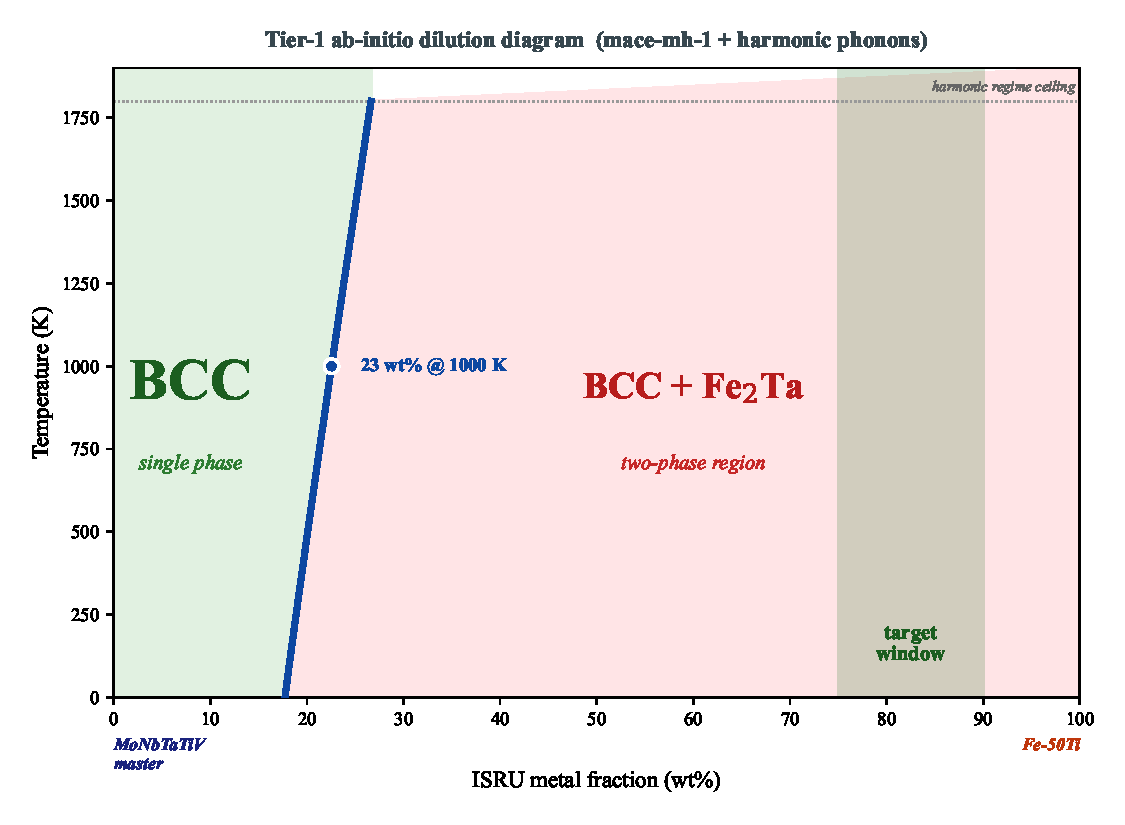
\includegraphics[width=0.85\textwidth]{figures/dilution_phase_diagram_v2.pdf}
\caption{Ab-initio Tier-1 dilution diagram (this work), drawn in the same visual layout as Figure~\ref{fig:dilution_diagram} for direct A/B comparison. Solid-state phase boundaries (Fe$_2$Ta cliff in blue, Fe$_2$Nb cliff in red dotted) are computed from the \texttt{mace-mh-1} foundation interatomic potential~\cite{Batatia2025MACEMH1} combined with harmonic phonopy phonons~\cite{Togo2015Phonopy} on the MoNbTaTiV $\rightarrow$ Fe-50Ti dilution path, with pure C14 Laves references (Fe$_2$Nb, Fe$_2$Ta). Liquidus and solidus on the Fe--Ti side are reproduced from literature; full TCHEA-grade $T$--$x$ remains future work. The 75--90~wt\% ISRU target window (green band) is past both computed cliffs at every temperature, supporting the qualitative picture in Figure~\ref{fig:dilution_diagram}.}
\label{fig:dilution_diagram_v2}
\end{figure}

% , Dual-Purpose Break-Even Comparison ,
\begin{figure}[p]
\centering

\includegraphics[width=\textwidth]{figures/dual_purpose_breakeven.pdf}
\caption{Break-even comparison: dead-weight cargo (top row) vs.\ dual-purpose mass (bottom row). \textbf{Left column:} IMLR~=~2 (50\% ISRU). \textbf{Right column:} IMLR~=~5 (80\% ISRU). In the dual-purpose model, the Earth-shipped refractory mass serves a primary structural function during transit and landing; its launch cost is fully amortised, eliminating the $C_L \cdot M_{\text{Earth}} \cdot N$ term from the cost model (Eq.~\ref{eq:total_cost_dual}). The resulting $C_L$ multiplier of $\text{IMLR}/(\text{IMLR}-1) > 1$ shifts the break-even boundary leftward and downward, expanding the viable green region into the low-launch-cost territory where the standard model predicts ISRU to be uneconomical.}
\label{fig:dual_purpose_breakeven}
\end{figure}

% , Manufacturing Pipeline Roadmap (4-lane swim-lane) ,
\begin{figure}[p]
\centering

\includegraphics[width=\textwidth]{figures/fig_manufacturing_roadmap.pdf}
\caption{End-to-end manufacturing pipeline for Earth-supplied refractory feedstock and ISRU-derived Fe--Ti / Al--Si streams. Four logistical lanes (Earth feedstock; ISRU feedstock; consolidation and quality control; validation) are mapped against three TRL stages: Stage~1 (TRL 3--5, laboratory ingot synthesis and densification), Stage~2 (TRL 5--6, surrogate-regolith ISRU substitution and full mechanical screening) and Stage~3 (TRL 6+, lunar pilot-line qualification against incumbents Inconel and Monel K500). Process windows on the diagram (mechanical alloying 40\,h heptane PCA; vacuum hot pressing 1\,500\,$^\circ$C / 2\,h / 30\,MPa for the refractory class, 1\,260\,$^\circ$C for the Ni-bearing high-entropy superalloy class; $\geq$98\,\% relative density; 9.4--12.9\,g/cm$^3$ bulk density envelope; ignition-rig acceptance at 180\,bar / 800\,K) are calibrated from this work's Phase~2 SPARK consolidation campaign and held constant across the ISRU substitution boundary.}
\label{fig:roadmap}
\end{figure}

% , XRD Panel (HESA + 8-element BCC + decomposition) ,
\begin{figure}[p]
\centering

\includegraphics[width=\textwidth]{figures/fig_xrd_panel.pdf}
\caption{XRD phase identification at three checkpoints of the SPARK consolidation pipeline (this work). \textbf{Left:} Ni-bearing high-entropy superalloy (HESA-class) compact, FCC matrix with minor MC carbide; \textbf{centre:} eight-element refractory variant, predominantly BCC with weak MC reflections; \textbf{right:} the same eight-element variant after a 1\,000\,$^\circ$C exposure, showing clear secondary-phase decomposition that drove its elimination from down-selection. Single-phase BCC was preserved in the down-selected refractory candidate (not shown; pattern consistent with the centre panel without the decomposition signature). XRD on the densified compact constitutes the consolidation-lane gate of Figure~\ref{fig:roadmap} and is the principal experimental anchor for the ab-initio phase-stability picture of Section~\ref{subsec:blending} and Figure~\ref{fig:dilution_diagram_v2}.}
\label{fig:xrd_panel}
\end{figure}

% , SPARK Alloy Landscape (HV2 + UTS bars) ,
\begin{figure}[p]
\centering

\includegraphics[width=\textwidth]{figures/fig_alloy_landscape.pdf}
\caption{SPARK programme alloy landscape (this work, Phase~2). \textbf{Top:} Vickers HV2 hardness on densified compacts. \textbf{Bottom:} mini-tensile ultimate tensile strength at room temperature (filled bars) and at 1\,000\,K (hatched bars). Compositions are anonymised under the SPARK designators (R1--R6 refractory, H1--H3 high-entropy superalloy, S1 Ni-baseline) consistent with the consortium IP envelope; the qualitative grouping (green = ductile single-phase, orange = mixed, red = brittle multi-phase) and the down-selection markers (\,*\,) are released. Two candidates survive the joint hardness--strength screen: one refractory BCC composition retaining UTS at 1\,000\,K, and one Ni-bearing FCC + MC composition with the highest absolute room-temperature strength of the campaign. These two carry forward into the strength-retention comparison of Figure~\ref{fig:strength_retention} and the validation lane of Figure~\ref{fig:roadmap}.}
\label{fig:alloy_landscape}
\end{figure}

% , Strength-Retention vs. Incumbents ,
\begin{figure}[p]
\centering

\includegraphics[width=0.85\textwidth]{figures/fig_strength_retention.pdf}
\caption{Strength retention of the two SPARK down-selected candidates (this work) against the incumbent reusable-engine baselines Inconel HP and Monel K500 across the room-temperature--1\,200\,K interval that brackets a methane-oxygen preburner working window (shaded). The down-selected refractory composition retains a substantially higher fraction of its room-temperature UTS at 1\,000\,K than either Ni-superalloy benchmark, while the down-selected Ni-bearing high-entropy variant matches Inconel HP in absolute strength at 1\,000\,K and exceeds it at room temperature. The 1\,000--1\,200\,K window is the principal Stage-3 acceptance band of the validation lane in Figure~\ref{fig:roadmap}.}
\label{fig:strength_retention}
\end{figure}

% , AM Temperature Field (top view) ,
\begin{figure}[p]
\centering
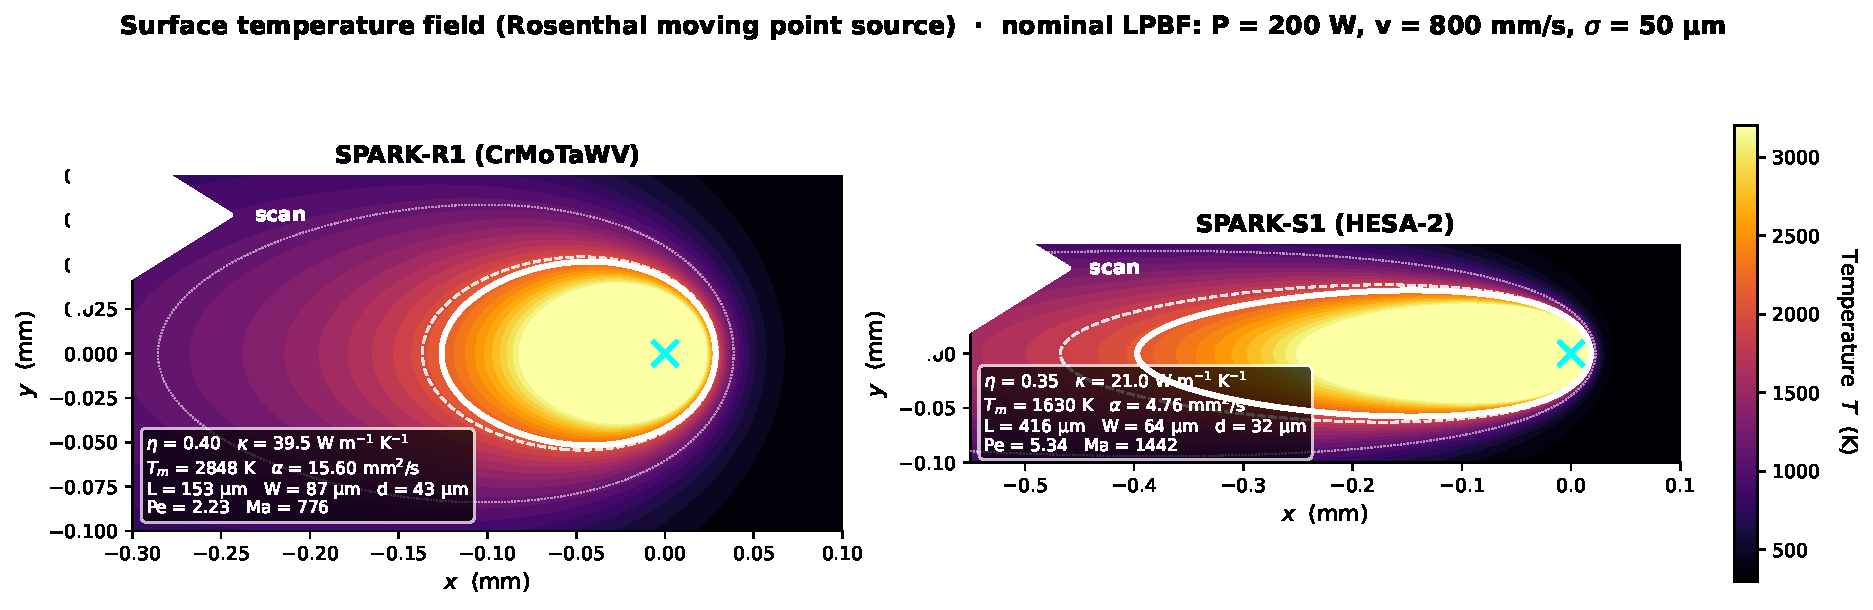
\includegraphics[width=\textwidth]{figures/fig_am_temperature_field.pdf}
\caption{Top-view temperature field $T(x,y,z=0)$ of the moving Rosenthal point source at the nominal LPBF point ($P = 200$\,W, $v = 0.8$\,m/s, $\sigma = 50\,\mu$m) for the two down-selected SPARK compositions (this work). The solid white isoline marks $T = T_m$; the dashed black isoline marks $T_m - 100$\,K. \textbf{Left:} SPARK-R1 (CrMoTaWV) produces a compact, near-circular melt pool (153\,$\mu$m long, 87\,$\mu$m wide) because the high thermal diffusivity ($\alpha = 1.56 \times 10^{-5}$\,m$^2$/s) lets heat run ahead of the laser. \textbf{Right:} SPARK-S1 (HESA-2) produces a markedly elongated comet shape (416\,$\mu$m long, 64\,$\mu$m wide) because the lower diffusivity ($\alpha = 4.76 \times 10^{-6}$\,m$^2$/s, a factor 3.3 below R1) traps the isotherm behind the moving spot. Scan direction is $+x$; the laser is at the origin. Field regularised at the source with $\varepsilon_R = 5\,\mu$m per Eq.~\ref{eq:rosenthal}.}
\label{fig:am_temperature_field}
\end{figure}

% , AM Cross-Section (longitudinal y=0 slice) ,
\begin{figure}[p]
\centering
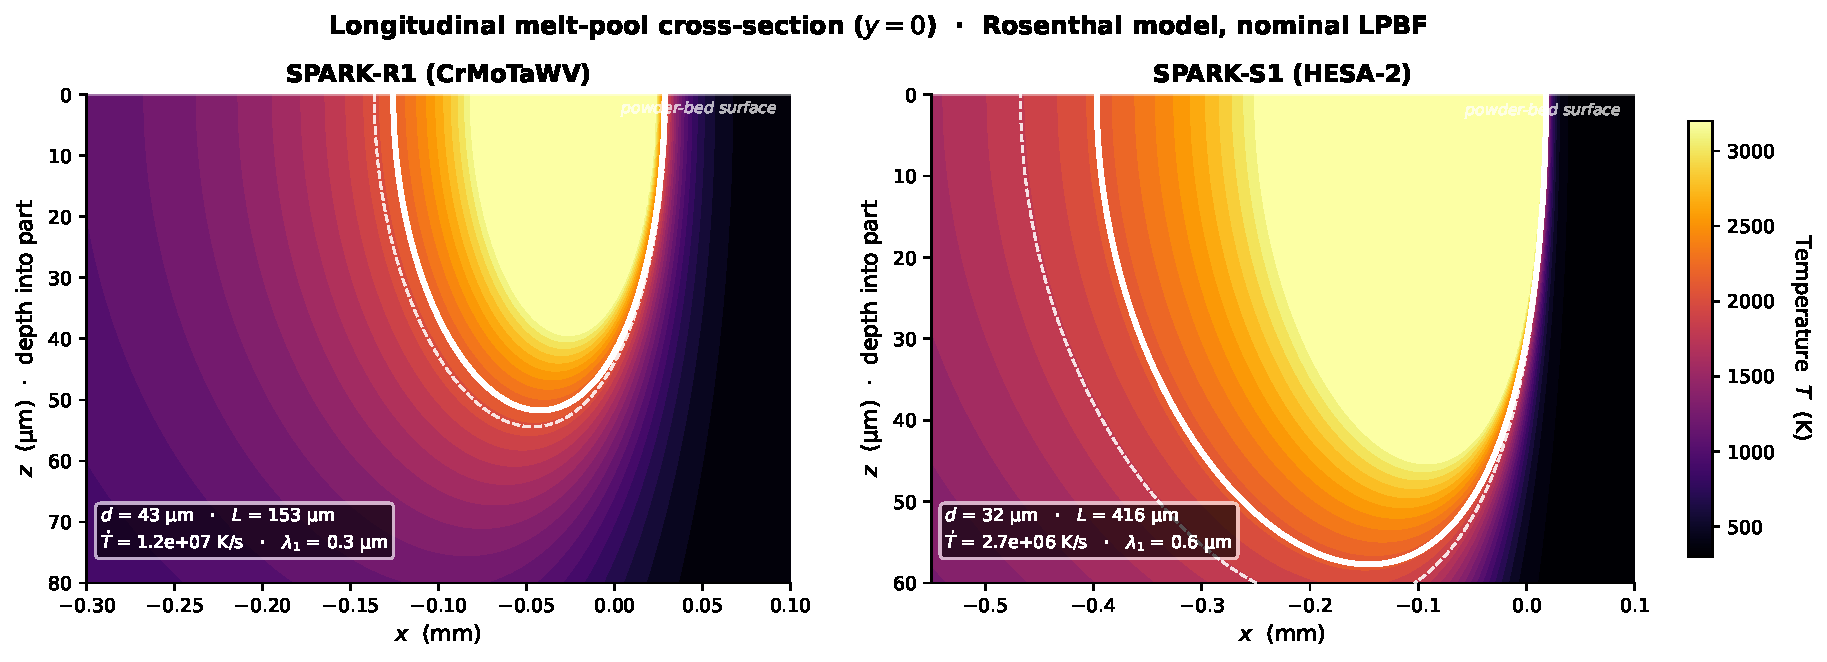
\includegraphics[width=\textwidth]{figures/fig_am_cross_section.pdf}
\caption{Longitudinal cross-section $T(x,y=0,z)$ of the Rosenthal melt pool at the nominal LPBF point (this work). The solid white curve is the $T_m$ isotherm; the dashed white curve is $T_m - 100$\,K. Pool depths $d$ are 43\,$\mu$m (SPARK-R1) and 32\,$\mu$m (SPARK-S1); both clear the 30\,$\mu$m layer-thickness threshold typical for LPBF of refractory and Ni-superalloy powders, so both alloys are predicted printable at the nominal point. The SPARK-S1 pool is visibly more elongated than R1's because of its lower thermal diffusivity (see Figure~\ref{fig:am_temperature_field}). Cooling rate $|\dot T|$ at the trailing-edge solidification front and predicted primary dendrite arm spacing $\lambda_1$ (Hunt 1979 / Kurz--Fisher~\cite{Hunt1979,KurzFisher1986}) are annotated for each alloy.}
\label{fig:am_cross_section}
\end{figure}

% , AM Process Map (P, v plane with d isolines) ,
\begin{figure}[p]
\centering
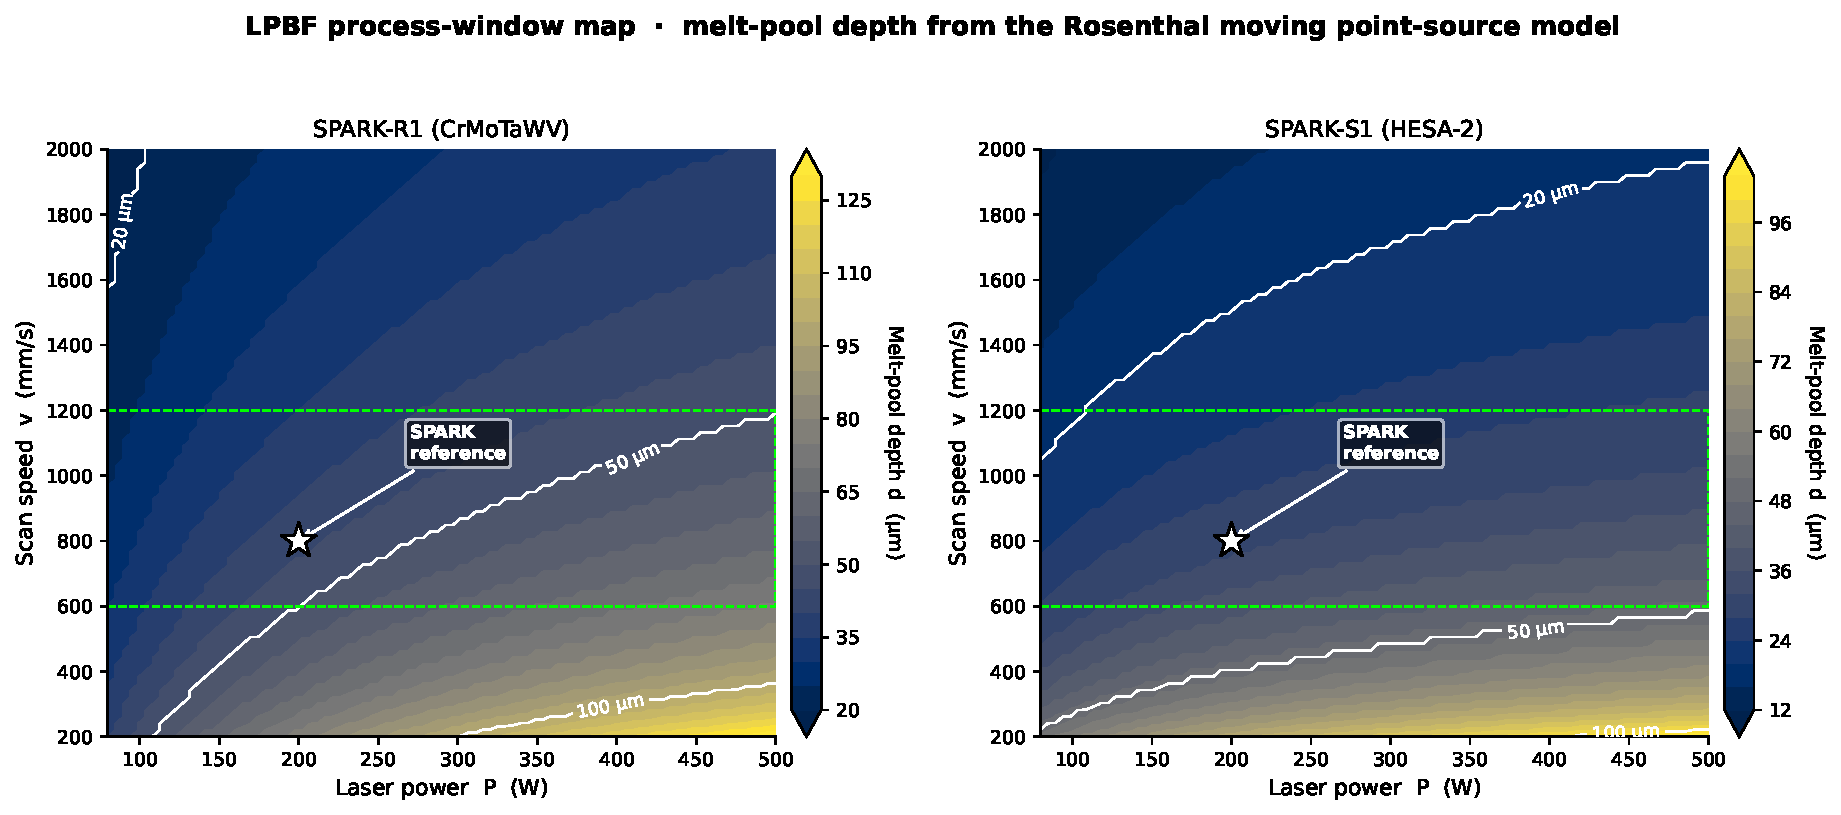
\includegraphics[width=\textwidth]{figures/fig_am_process_map.pdf}
\caption{Melt-pool depth $d$ as a function of laser power $P$ and scan speed $v$ for the two SPARK down-selected compositions, computed on a 90$\times$90 grid in $(P,v)$ space from the Rosenthal field of Eq.~\ref{eq:rosenthal} (this work). The bold black contour is the 30\,$\mu$m printability isoline; the dashed contour is 60\,$\mu$m (deep-pool regime). The nominal SPARK process point ($P = 200$\,W, $v = 0.8$\,m/s, white star) sits well above the printability isoline for SPARK-R1 and just above it for SPARK-S1, indicating comfortable margin for the refractory candidate and a tighter qualification window for the Ni-bearing candidate. The hyperbolic shape of the isoline ($P/v \approx$ const) is characteristic of conduction-mode LPBF and falls out of the moving-point-source field by inspection of Eq.~\ref{eq:rosenthal}.}
\label{fig:am_process_map}
\end{figure}

% , AM Sensitivity Tornado ,
\begin{figure}[p]
\centering
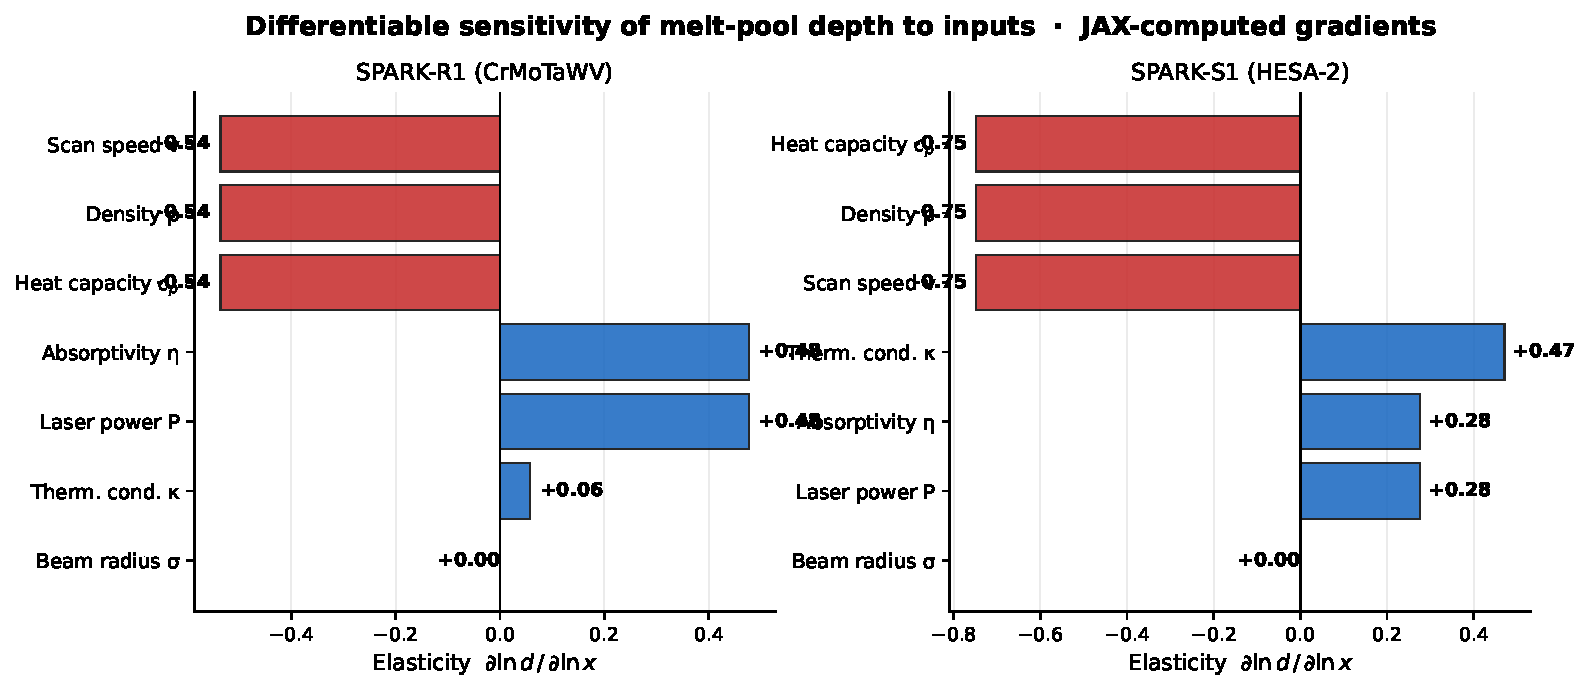
\includegraphics[width=0.85\textwidth]{figures/fig_am_sensitivity.pdf}
\caption{Engineering depth elasticities $E_p = (p/d)\,\partial d/\partial p$ for the two SPARK down-selected compositions at the nominal LPBF point, derived by automatic differentiation of the Rosenthal field through the implicit-function theorem (Eq.~\ref{eq:elasticity}; this work). The chain rule through $\alpha = \kappa/(\rho c_p)$ is applied so that $\eta$, $P$, $v$, $\kappa$, $\rho$, $c_p$, and the beam radius $\sigma$ are treated as physically independent inputs. Sign convention: positive elasticity (red) deepens the pool, negative (blue) shrinks it. Signs are identical for both alloys and physically transparent; magnitudes separate cleanly. SPARK-S1 carries $|E| \approx 0.76$ on $v$, $\rho$, and $c_p$,roughly 50\,\% above the SPARK-R1 sensitivities,which translates into a tighter incoming-powder-quality window for the Ni-bearing alloy. The $\sigma$ elasticity is zero by construction in the regularised point-source limit.}
\label{fig:am_sensitivity}
\end{figure}

% , AM Lunar Dimensionless Numbers ,
\begin{figure}[p]
\centering
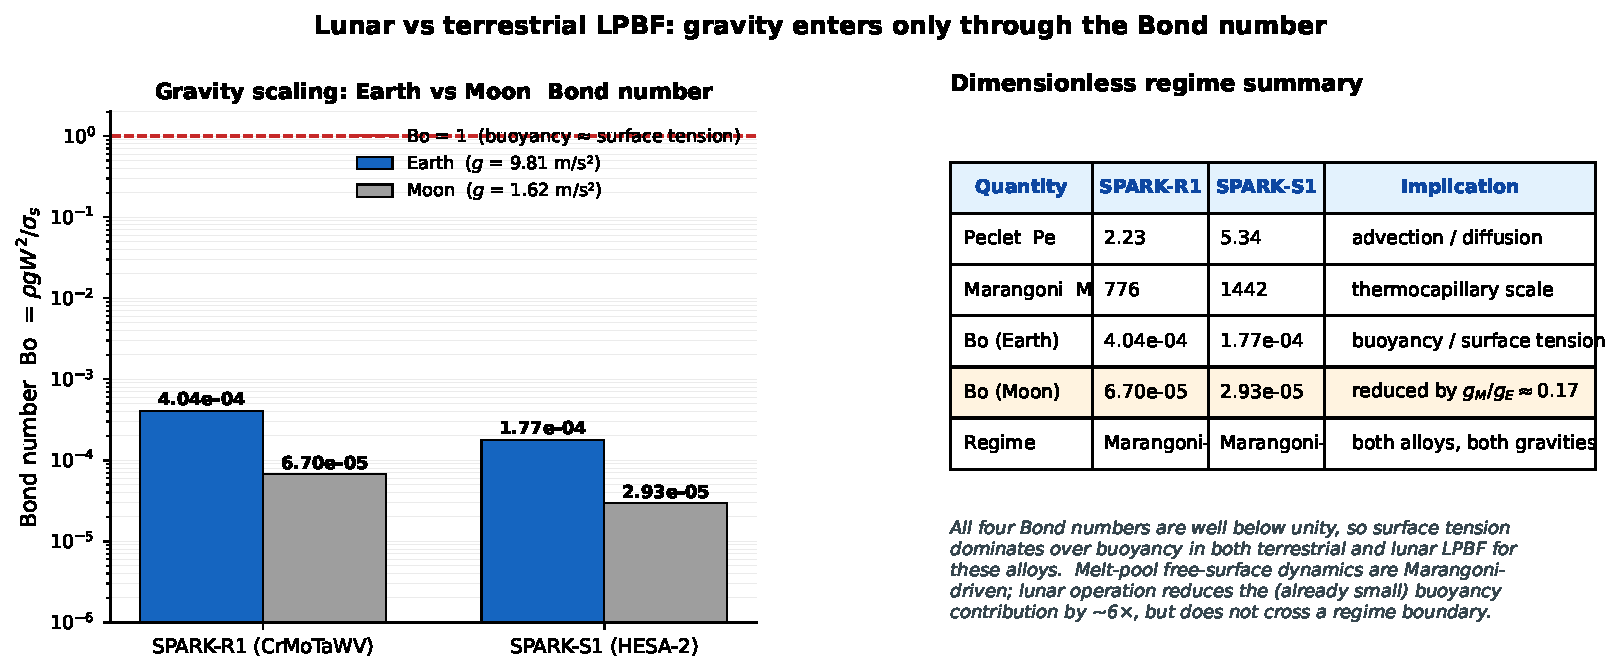
\includegraphics[width=\textwidth]{figures/fig_am_lunar_dimensionless.pdf}
\caption{Dimensionless analysis of the LPBF melt pool for the two SPARK candidates at Earth gravity ($g = 9.81$\,m/s$^2$) and lunar gravity ($g = 1.624$\,m/s$^2$). \textbf{Peclet} $\mathrm{Pe} = vW/(2\alpha)$ and \textbf{Marangoni} $\mathrm{Ma} = |d\sigma/dT|\,\Delta T\,W/(\rho\nu_l\alpha)$ are gravity-independent and identical at the two gravities; both alloys sit in the Peclet-elongated, strongly Marangoni-stirred regime. \textbf{Bond} $\mathrm{Bo} = \rho g W^2 / \sigma_s$ is the only gravity-coupled number: dropping from $4.04 \times 10^{-4}$ (R1, Earth) to $6.70 \times 10^{-5}$ (R1, Moon) and from $1.77 \times 10^{-4}$ (S1, Earth) to $2.93 \times 10^{-5}$ (S1, Moon). All four values are 4--5 decades below the Bo $= 1$ surface-tension threshold (red dashed line), so surface tension dominates pool morphology by a wide margin under both gravities. Gravity-dependent physics in lunar AM is confined to the powder layer outside the pool (recoater spreading, spatter, debris evacuation), not the pool itself.}
\label{fig:am_lunar_dimensionless}
\end{figure}

% , AM Lunar Terrane-Resolved Screen (bar chart) ,
\begin{figure}[p]
\centering
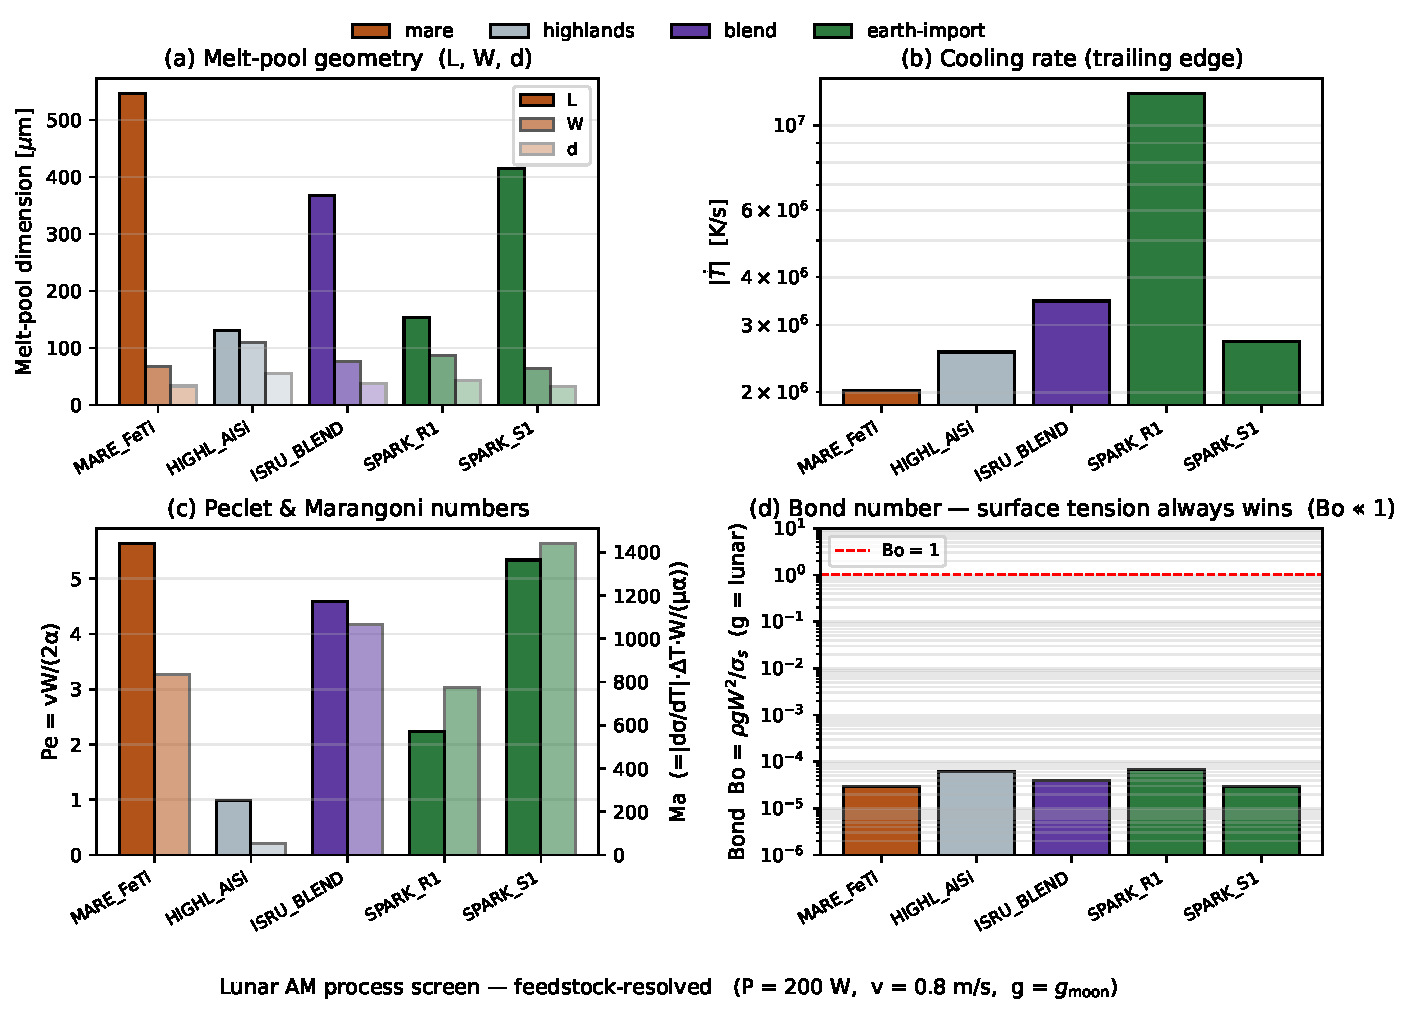
\includegraphics[width=\textwidth]{figures/fig_lunar_terranes_bars.pdf}
\caption{Lunar-terrane-resolved AM screen at the nominal LPBF point under lunar gravity (this work). Colour groups: orange = mare-derived Fe--Ti, grey = highlands-derived Al--Si, purple = ISRU cross-terrane blend Fe$_{0.3}$Ti$_{0.3}$Al$_{0.2}$Nb$_{0.1}$Ta$_{0.1}$ with MACE-supplied density ($\rho = 7\,172$\,kg/m$^3$), green = Earth-imported SPARK compositions. \textbf{(a)} Melt-pool length $L$, surface width $W$ and depth $d$ in microns; all five alloys clear the 30\,$\mu$m printability threshold. \textbf{(b)} Cooling rate $|\dot T|$ at the trailing edge (log scale): SPARK-R1 sits an order of magnitude above the lunar feedstocks because of its high $\kappa\,\Delta T$ product, predicting commensurately finer dendrite spacing. \textbf{(c)} Peclet (left axis) and Marangoni (right axis) numbers: highlands Al--Si is the only alloy in the near-spherical (Pe $\approx 1$) regime; the other four are Peclet-elongated. \textbf{(d)} Bond number on a log scale: all five alloys are 4--5 decades below the Bo $= 1$ surface-tension threshold (red dashed), confirming gravity-independent pool morphology across every terrane-resolved chemistry. Quantitative values in Table~\ref{tab:lunar_terrane_am}.}
\label{fig:am_lunar_terrane}
\end{figure}

\end{document}
